% !TEX root = ../../book.tex
\chapter{Execution Strategies\label{chap:ch_exec_models}}

We finally turn our discussion to one of the central characters in this book if not the absolute starring. Execution strategies are arguably the core mean by which capital flows in and out of the financial markets.  As discussed in Chapter~\ref{chap:ch_trading_fund} large money managers, mutual fund companies and hedge funds have large holdings (some have AUMs in the trillions of dollars) and are in constant need to trade in order to re-balance their portfolios to achieve their investment objectives and to manage inflows and  outflows of capital. These trades are usually large with respect to the instantaneously available  in the market at reasonable prices. This forces the trader to slice the order in smaller, sizable chunks that are more easily absorbed by the market; They also need to skillfully trade these slices as to minimize the footprint left in the market under the form of market impact. Started as nothing more than utilities tools to implement the simpler trades the field has ballooned into a multi-billion dollar industry where a large number of sell side brokers as well as fintech driven companies are fiercely competing for a piece of the pie. In a way that sadly seems typical in other endeavors in finance the execution space evolved in a somewhat chaotic space full of misinformation, marketing fads, gimmicks, and in many cases misunderstandings. Albeit slowly the field is maturing and is starting to focus on the real core aspects of this problem and applying new ideas and innovative approach and we expect the field to go through a sort of a new golden age in the coming years.


In this chapter, we will follow the usual path of starting with a practitioner view of the field, the core components, and the approaches being used in practice. We will walk through a brief history and underlying ideas behind the current product line and a more in depth treatment of the current state of affair. We will strive to dispel as many of the misconceptions we feel still exist in the understanding of the core principles underlying the various approaches providing a somewhat unique treatment that might be considered controversial by some of our peers and clients alike but that we feel to be closer to reality encouraging the interested readers to approach the field with new eyes focusing on the things that really matter and on the many problems that still need to be solved.


The second part will take the treatment to a more formal quantitative level providing the evolution of the research area named ``Optimal Execution'' and the author's view on the modeling approaches that will comprise the next generation Execution product.



% Introduction to Execution
\section{Introduction to Execution}


Execution generally refers to a branch of Algorithmic Trading that is concerned with  implementing, as efficiently as possible, an investment decision of a portfolio manager (PM). That investment decision can be summarized as: the instrument to transact, the direction (buy or sell) and the quantity (how many shares or contracts). It also often includes additional trading instructions to support the trader in his decision on how to trade the particular order like for example the maximum (minimum) price she is willing to buy (sell). 


As such, unlike other algorithmic trading strategies we have discussed in previous chapters, WHAT to trade is exogenous to the strategy which is only concerned on HOW to best trade the order. In addition to the PM directed parameters the strategy will need additional  required parameters: Start Time, and End Time. These parameters determine when the strategy can start trading and when it needs to stop. The Start Time is a low bound not necessarily the exact time when the strategy will start trading, similarly the End Time is an upper band on the time but the strategy could stop trading earlier than that. Finally there is a whole set of additional supported parameters some general (e.g. maximum participation rate, limit price) and some strategy specific that provide the constraints the strategy will need to abide to essentially limiting the ``Solution Space'' available to the strategy.
As stated before in most relevant cases the order to be executed is too large for the market to absorb as a whole so the order will generally need to be sliced in some form or another. Execution strategies provide different approaches to this slicing to try to achieve the trader's particular objective.


At this point we are going to start deviating from other treatments of the subject. The standard treatment would at this point introduce various benchmarks (mostly some form prices but could also be a participation rate) that essentially codify the objective of the strategy and algorithmic trading strategy evolved to minimize the distance to that benchmark. This is in our opinion a revisionist view on how algorithmic trading evolved and a misconception that still mires the industry. Do trader have different objectives? Are they really trying to achieve certain benchmarks? The answer is mostly No. The objective of the trader is always to get the ``best price'' possible for the particular order within the constraints given to her by the PM. The problem is that the ``best price''  is an unknown ex-ante and worse than that it's unknowable. Unknowable because the choice of the trader will change the path of the price and volume evolution thus there is no way to know how that price would have evolved had the trader done something else. So execution strategies evolved to approach the problem in  different ways  and in order to provide the trader with ways to express their views in more an more sophisticated ways on how to maximize the chance to achieve that elusive best price.



% Benchmarks
\subsection{Benchmarks}

Once the approach has been defined the outcome will need to be measured to have a view of how well the trader did. The standard benchmark to measure a trading outcome is the ``Implementation Shortfall'' (IS). This the execution price compared to the ``prevailing'' price at the time the trader received the order \footnote{From a PM perspective the Implementation Shortfall is against the prevailing price at the time the decision was made. In this book we take the Trader perspective}. Formally:
        \begin{equation}
        \text{IS} = \text{side}\, \frac{p_{\text{exec}} - p_{\text{arrival}}}{p_{\text{arrival}}},
        \end{equation}
where `side' is the side multiplier: $1$ for buys $-1$ for sells, $p_{\text{exec}}$ is the execution price achieved and $p_{\text{arrival}}$ is the prevailing price at order arrival. This is usually the mid point at time of arrival but could also be the last traded price before the order arrived.\footnote{Theses choices while seemingly benign are actually somewhat tricky as they can lead, in some fringe cases, to significant measurement outliers. Think for example if right before the order the spread gaps for a short moment leading the mid point to be very different than what one would call prevailing price. Alternatively on less liquid stock that don't trade often, the last traded price might be several minutes old the the prevailing price might have moved significantly.}


Implementation Shortfall is the most sensible choice because it is related to trading P\&L achieved during the trade.  It suffers however from several drawbacks:

\begin{itemize}
\item This benchmark captures the effects of the particular trading activity (i.e. market impact) that are due to the trading approach chosen but also the exogenous price diffusion due to alpha embedded in the investment decision and the activity of other participants. In most cases the exogenous effects are much larger than the endogenous ones and even on the endogenous side the more significant components are not under the control of the strategy and are dependent on the exogenous order characteristics and choice of approach. This makes Implementation Shortfall not well suited to understand how well the strategy is working.

\item The IS benchmark attributes special meaning to the $p_{\text{arrival}}$ anchor price. This led to a widespread belief that in order to minimize the slippage vs arrival one should adjust the trading approach as prices deviate either in favor or against the   $p_{\text{arrival}}$. Lacking any additional information and under a weak market efficiency assumption this is clearly erroneous as the strategy would make decision based on spurious noise leading to a much wider distribution of outcomes.

\item This benchmarks tells us little on how close the trade was to the ``best price'' and thus, on it's own does not provide any additional support on how to improve the particular trading approach
\end{itemize}


For this reason early practitioners started using benchmarks meant to measure how well the strategy implemented the particular approach of trading. The strategy name took the name of the benchmark it tries to achieve. One cannot talk about the benchmark without discussing, at a high level, the approach taken by the  eponymous strategy.


This approach, while sensible, had unintended consequences we are still facing today to some extent. Early users and sellers of these algorithms started equating the benchmark and the strategy used to achieve it as the actual ultimate objective of the strategy and that these strategies should not be used if a trader has an IS benchmark, which arguably any trader ultimately has. Our claim is that all these strategies are IS strategies that, when no better information around price direction/dynamics exist, are focusing on trying to minimize impact by managing the realized trading rate which, as we know, is the most understood driver of market impact.


Let's review the basic benchmarks and related strategies. \\


\noindent\emph{TWAP} \\


The Trade Weighted Average Price (TWAP) is the simplest of all the benchmarks and is simply the simple average price of every trade over the time horizon. 
        \begin{equation}
        \text{TWAP}_{\text{st}} ^{\text{et}}= \frac{1}{N}\sum_{i=0}^N{p_i}.
        \end{equation}
While very simple this benchmark tries to compare the price with the prices achieved by other participants over the time horizon allotted. It's essentially a measure of mediocrity but it's at least stable and corrects for the exogenous price moves and is thus much more stable over time. That being said it also has several downsides. As a benchmark TWAP is unknown until the end of execution (each trade in the market changes the value of the benchmark, contrary to the arrival price). It is also directly impacted by one's trades (they count toward the TWAP market price) and thus not really an independent benchmark and could be manipulated. This benchmark is rarely used today being superseded by VWAP which we discuss in the next paragraph.


This TWAP strategy, is the embodiment of the simplest way to split a large order: equally slice the order over the available time. Technically if wanted to achieve the best trade weighted price one would want to trade more when there are more trades but early algo designers probably did not really spent too much time thinking about it and it never felt important enough to actually implement it correctly.


It is hard to argue that there is anything optimal in this approach but lacking any other information and knowledge about the behavior of price and volume it would be one of the only alternative when completing the order is a requirement. We'll see below an arguably better approach if order completion is not required. 


While very simple TWAP is still used in particular in some less developed markets, it's also used by some systematic quantitative strategy where the joint trading schedule of a long-short portfolio is optimized as part of the investment strategy and then each individual short term slice (5--15~m) is sent to a TWAP algorithm. This will help maintain the dollar neutrality of the portfolio. \\

        \begin{figure}[!ht]
        \centering
        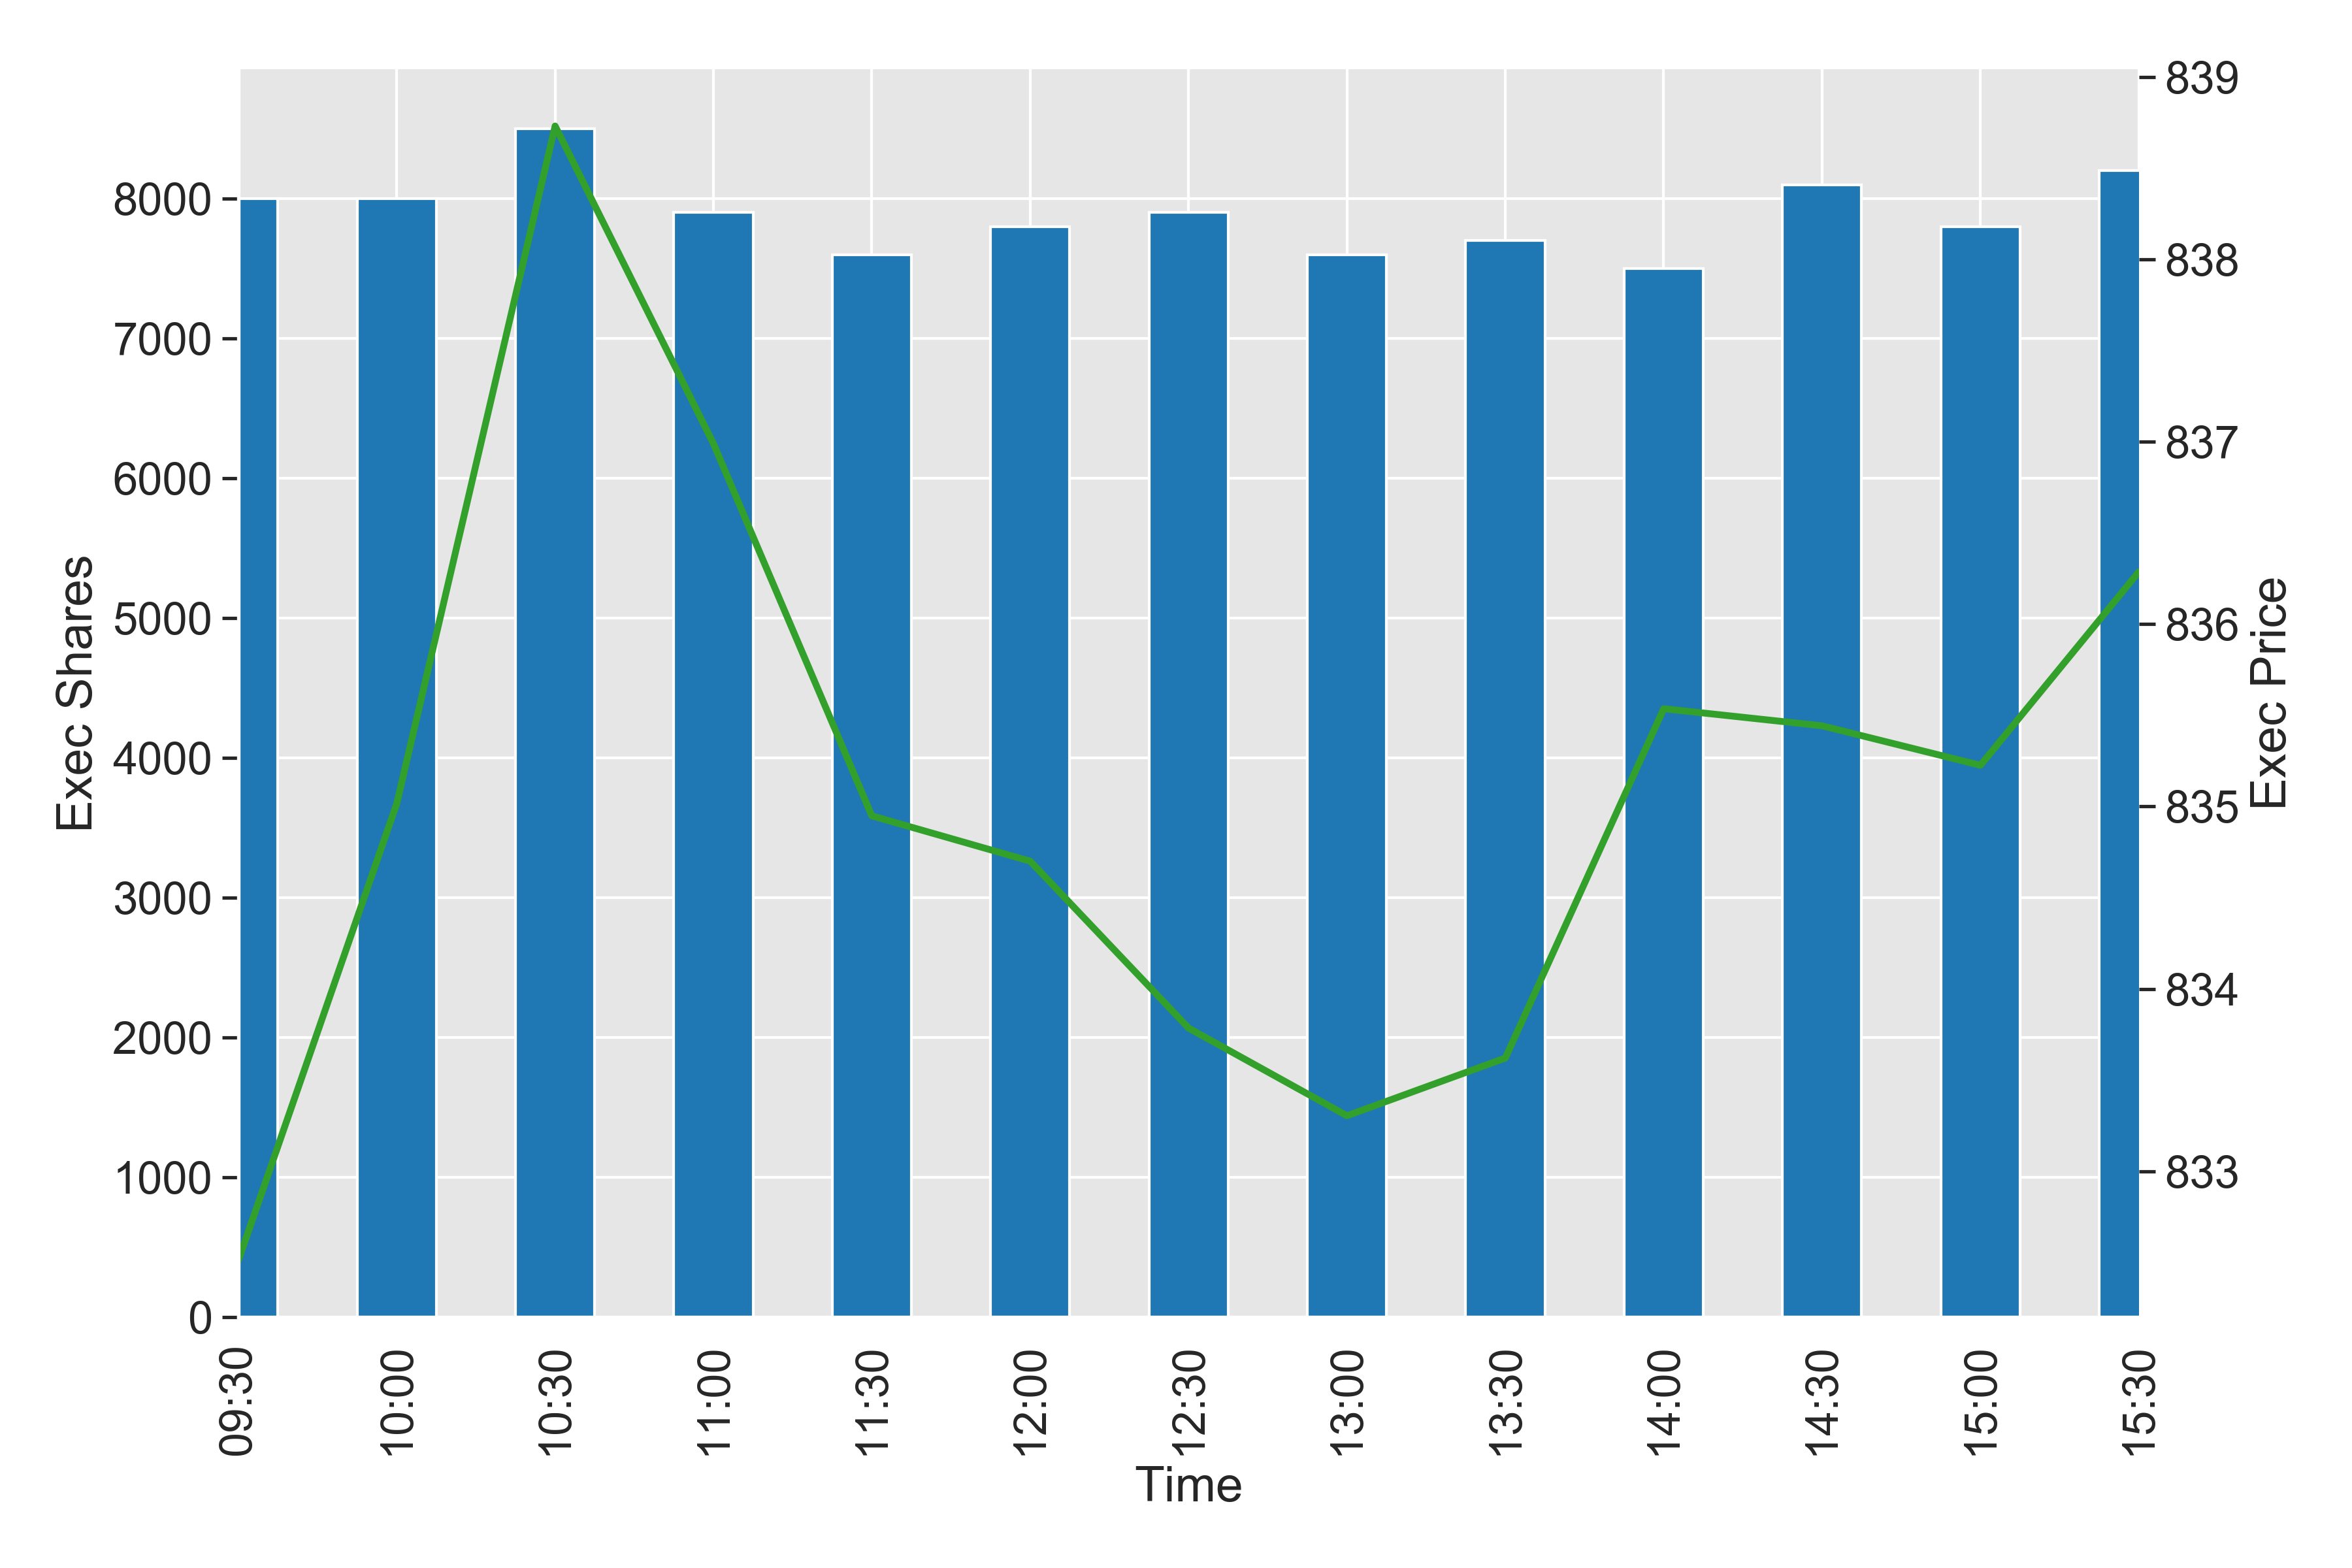
\includegraphics[width=0.75\textwidth]{chapters/chapter_exec_models/figures/twap.png} 
        \caption{Example of TWAP Trade for AMZN \label{fig:vwap}}
        \end{figure}


\noindent\emph{VWAP:} 


The Volume Weighted Average Price (VWAP) is the next simplest benchmark. Simply weight every trade by the normalized trade size.
        \begin{equation}
        \text{VWAP}_{\text{st}} ^{\text{et}}= \dfrac{ \sum_{i=0}^N p_i^* s_i }{ \sum_{i=0}^N s_i }.
        \end{equation}
This benchmark  is arguably a better measure of the fair market price over the period (trading a times and prices that are closer to the times and prices other market participants - who might have a better assessment of the short term price - trade). All the arguments for and against the VWAP benchmark are the same as the ones discussed for TWAP.


The VWAP strategy, in order to achieve its goal, takes advantage of the relative stability of the volume distribution over the day we discussed in Section~\ref{s:profiles}. Instead of trading equally throughout the time period is splits the order proportionally to the volume profile re-normalized over the time horizon.


The VWAP strategy is conceptually superior to TWAP as a market impact reduction approach since by trading more (less) when more  (less) volume is expected to trade it does a better job ad minimizing the realized trading rate. That being said if the volume profile is extremely noisy or unpredictable because of special circumstances trading VWAP might actually be inferior to TWAP since the error in our volume profile prediction might cause the strategy to achieve a higher trading rate than the simpler strategy.


There is an argument to be made that, reiterating the lack of any price dynamic/prediction information, VWAP is the best approach to trade an order when the order needs to complete. For this reason the strategy is still one of the most used strategy by quantitatively driven funds in which the investment strategy correctly sizes the order to minimize overall impact. 


Generally, while in recent years the popularity of VWAP has decreased in favor of the more flashy ``Liquidity Seeking'' strategies, this approach is still one of the most used strategy in the market. We'll discuss Liquidity Seeking strategies in a later section. \\


        \begin{figure}[!ht]
        \centering
        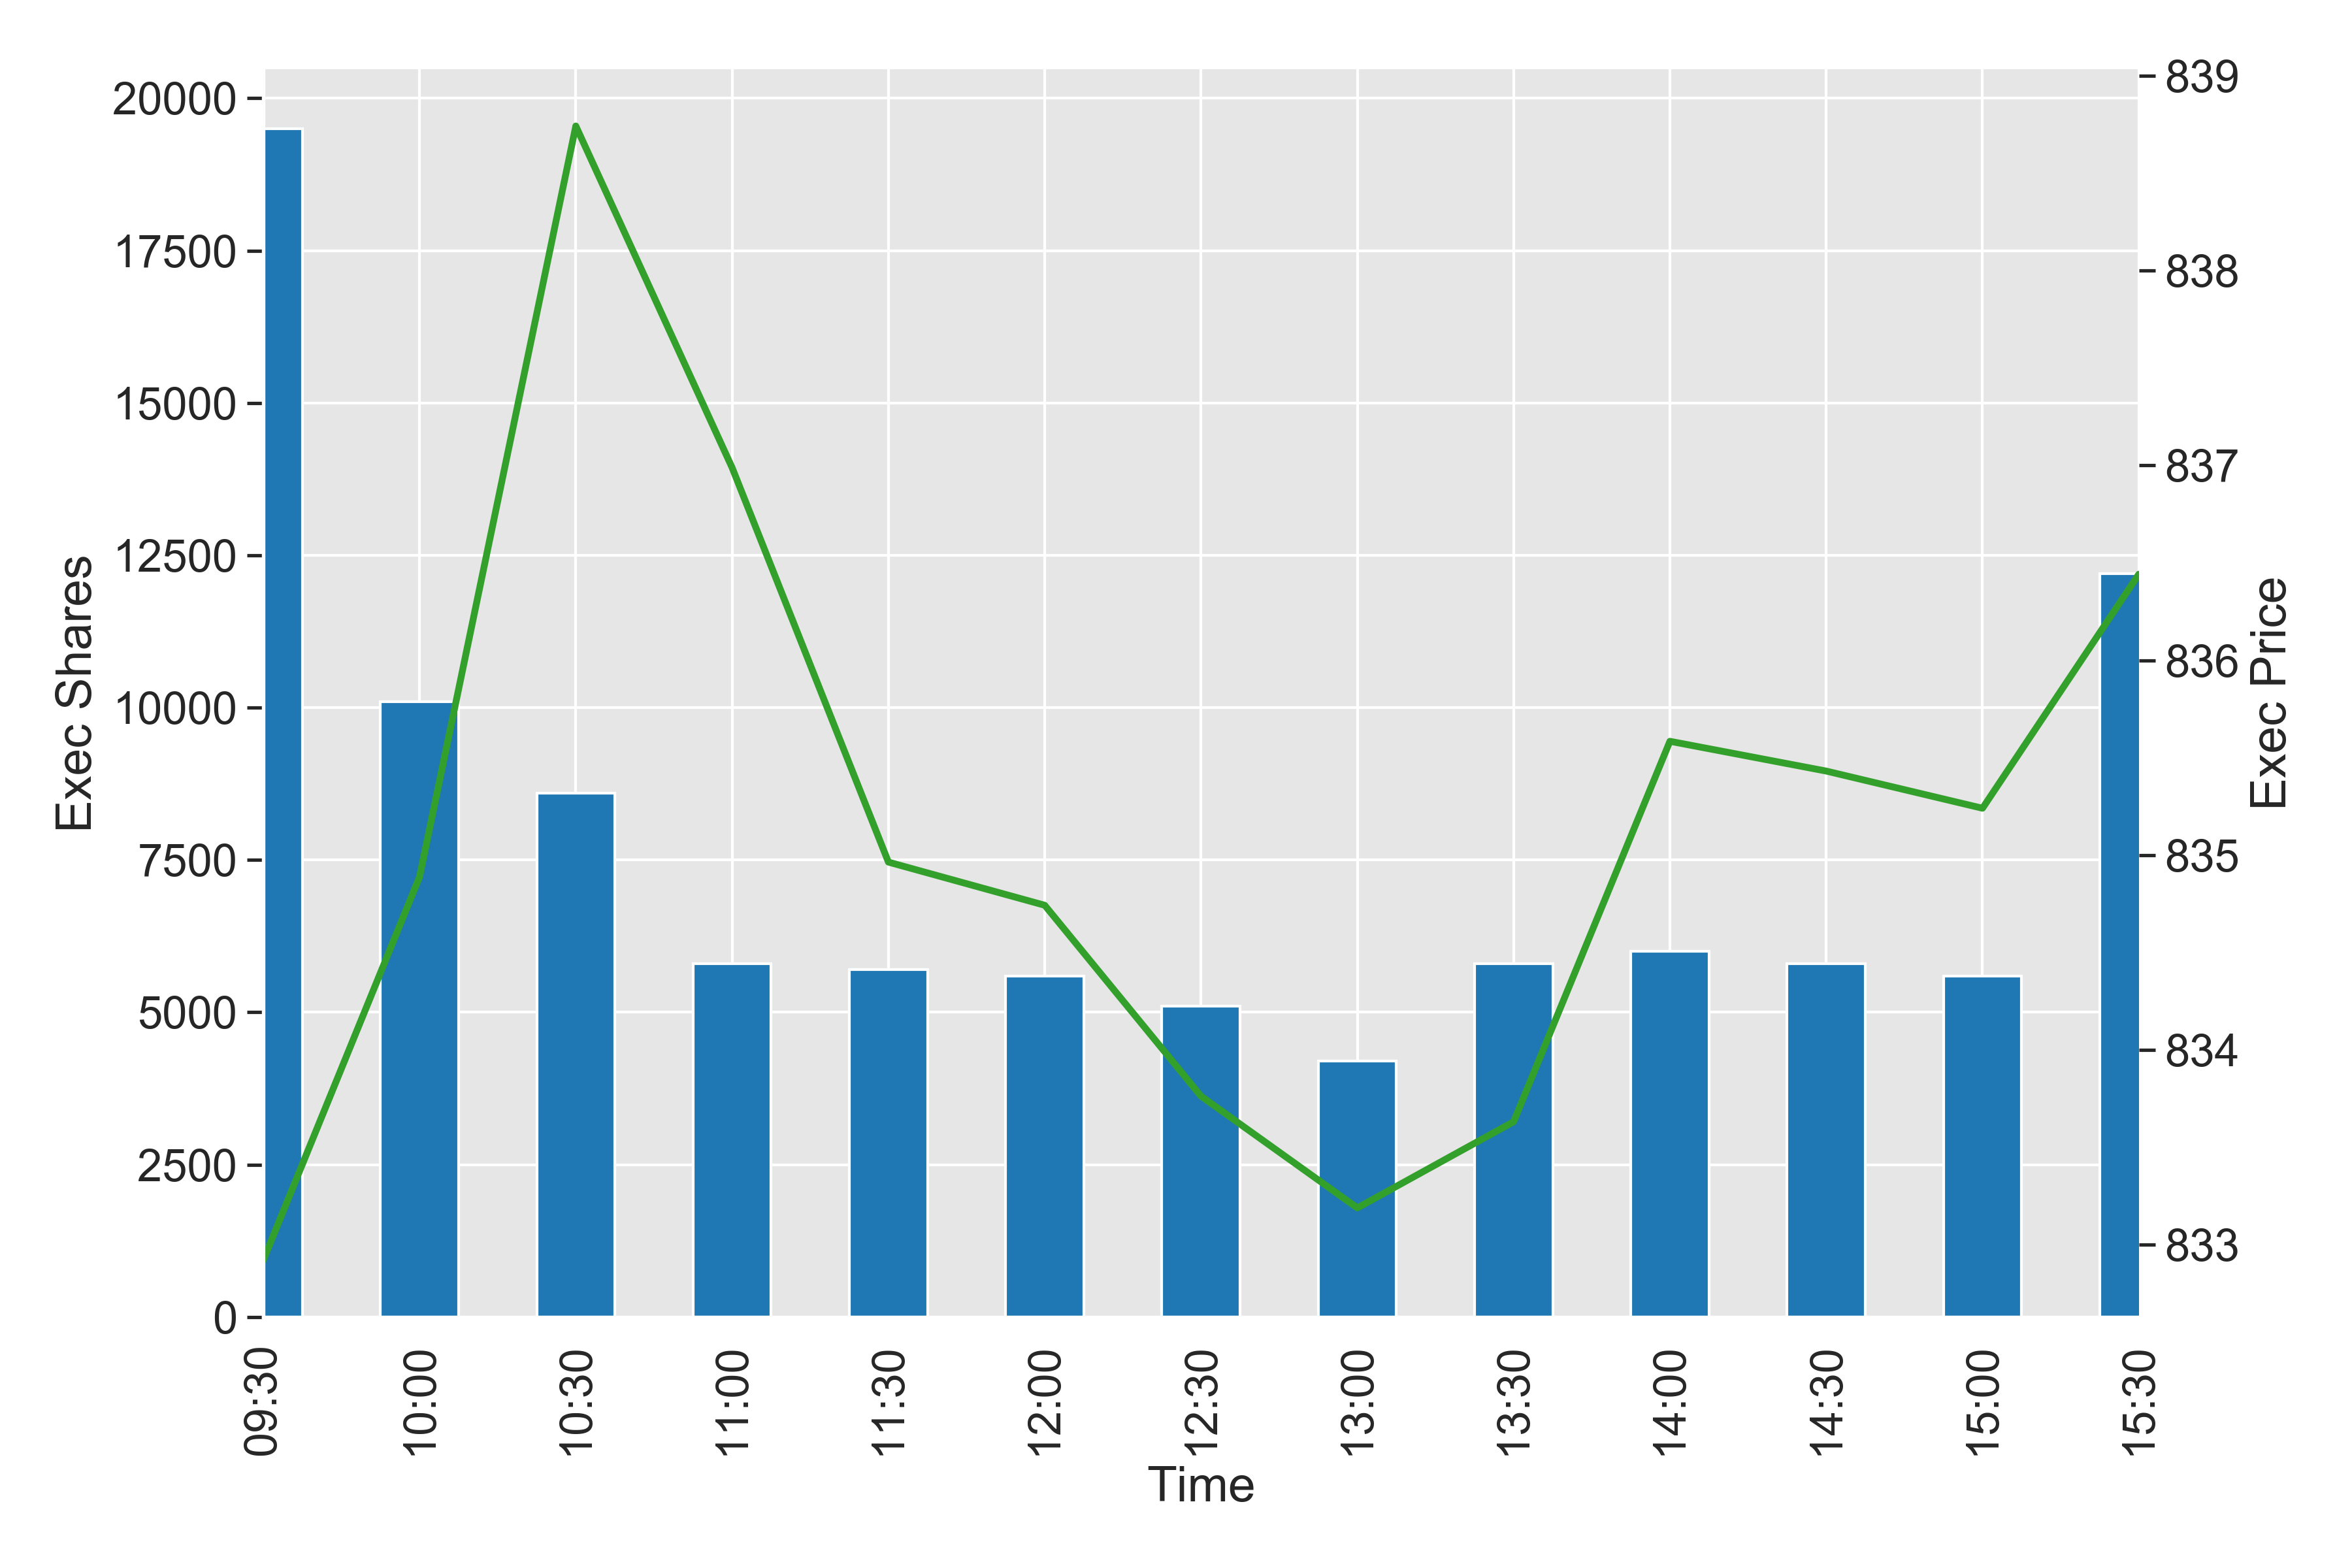
\includegraphics[width=0.75\textwidth]{chapters/chapter_exec_models/figures/vwap.png} 
        \caption{Example of VWAP Trade for AMZN\label{fig:vwap}}
        \end{figure}


\noindent\emph{Inline with Volume aka POV:} \\


The previous paragraph hinted that one of the limitation of VWAP (and TWAP) as a market impact controlling approach is that id does not take into consideration the high degree of volatility of the daily volume. If in a particular day the volume is significantly less than expected over the time horizon (due to lack of activity or large distortion in the volume profile) the VWAP strategy will just trade at a higher rate than envisioned by the trader leading to a higher total cost. Conversely If a trader who is trading a multiday order is too conservative and in that day there is a lot more volume than expected, she might trade a smaller portion of the order than the market would have been able to absorb.


If completing the order is an absolute hard necessity, arguably, there is little that can be done however if there is some flexibility then another approach can be taken. This is where Inline strategies come into play. Inline or alternatively called POV (Percentage of Volume) strategies have a benchmark that is not a price but a target trading rate. They aim at trading at a fixed rate as a way to directly control market impact. While seemingly straightforward, following a certain participation rate is not at all an easy task and these strategies can have some severe drawbacks unless carefully implemented.


\begin{itemize}
\item Early implementation where purely reactive meaning they would observe volume for a certain period and then trade the proscribed portion of that volume in the next iteration. Due to the noise in the volume dynamics this could lead the strategy to oversize the market after in the period after a large volume period. In particular large block prints if not correctly managed can cause the strategy to severely over-trade

\item Even when a volume forecast is used there is still a lot of error in the estimates and any shortfall needs to correctly managed and possibly smoothed over multiple periods to avoid excessive impact.

\item The POV benchmark is extremely noisy at the beginning of the order due to the granularity of trading which could lead to no trading at the beginning until enough volume as traded and then immediately chasing that volume aggressively because immediately well behind the target volume.
\end{itemize}


Because of these drawbacks and complexities Inline strategies have somewhat lost their popularity and the more flexible Liquidity Seeking approaches  have more or less sub-plant them.


The POV benchmark does not provide a way to measure effectiveness of the strategy as an impact prevention approach in particular because of the issues discussed above. The PWP $X$ (Participation Weighted Price at $X$\% of the market) price is used as a measure of execution quality for the inline benchmark. It represents the price one would have obtained had they traded $X$\% of the market volume until completion of the order (in practice, the VWAP of the period from order start until ($1/X \times$ Order Size) has traded in the market).

	\begin{figure}[!ht]
	\centering
	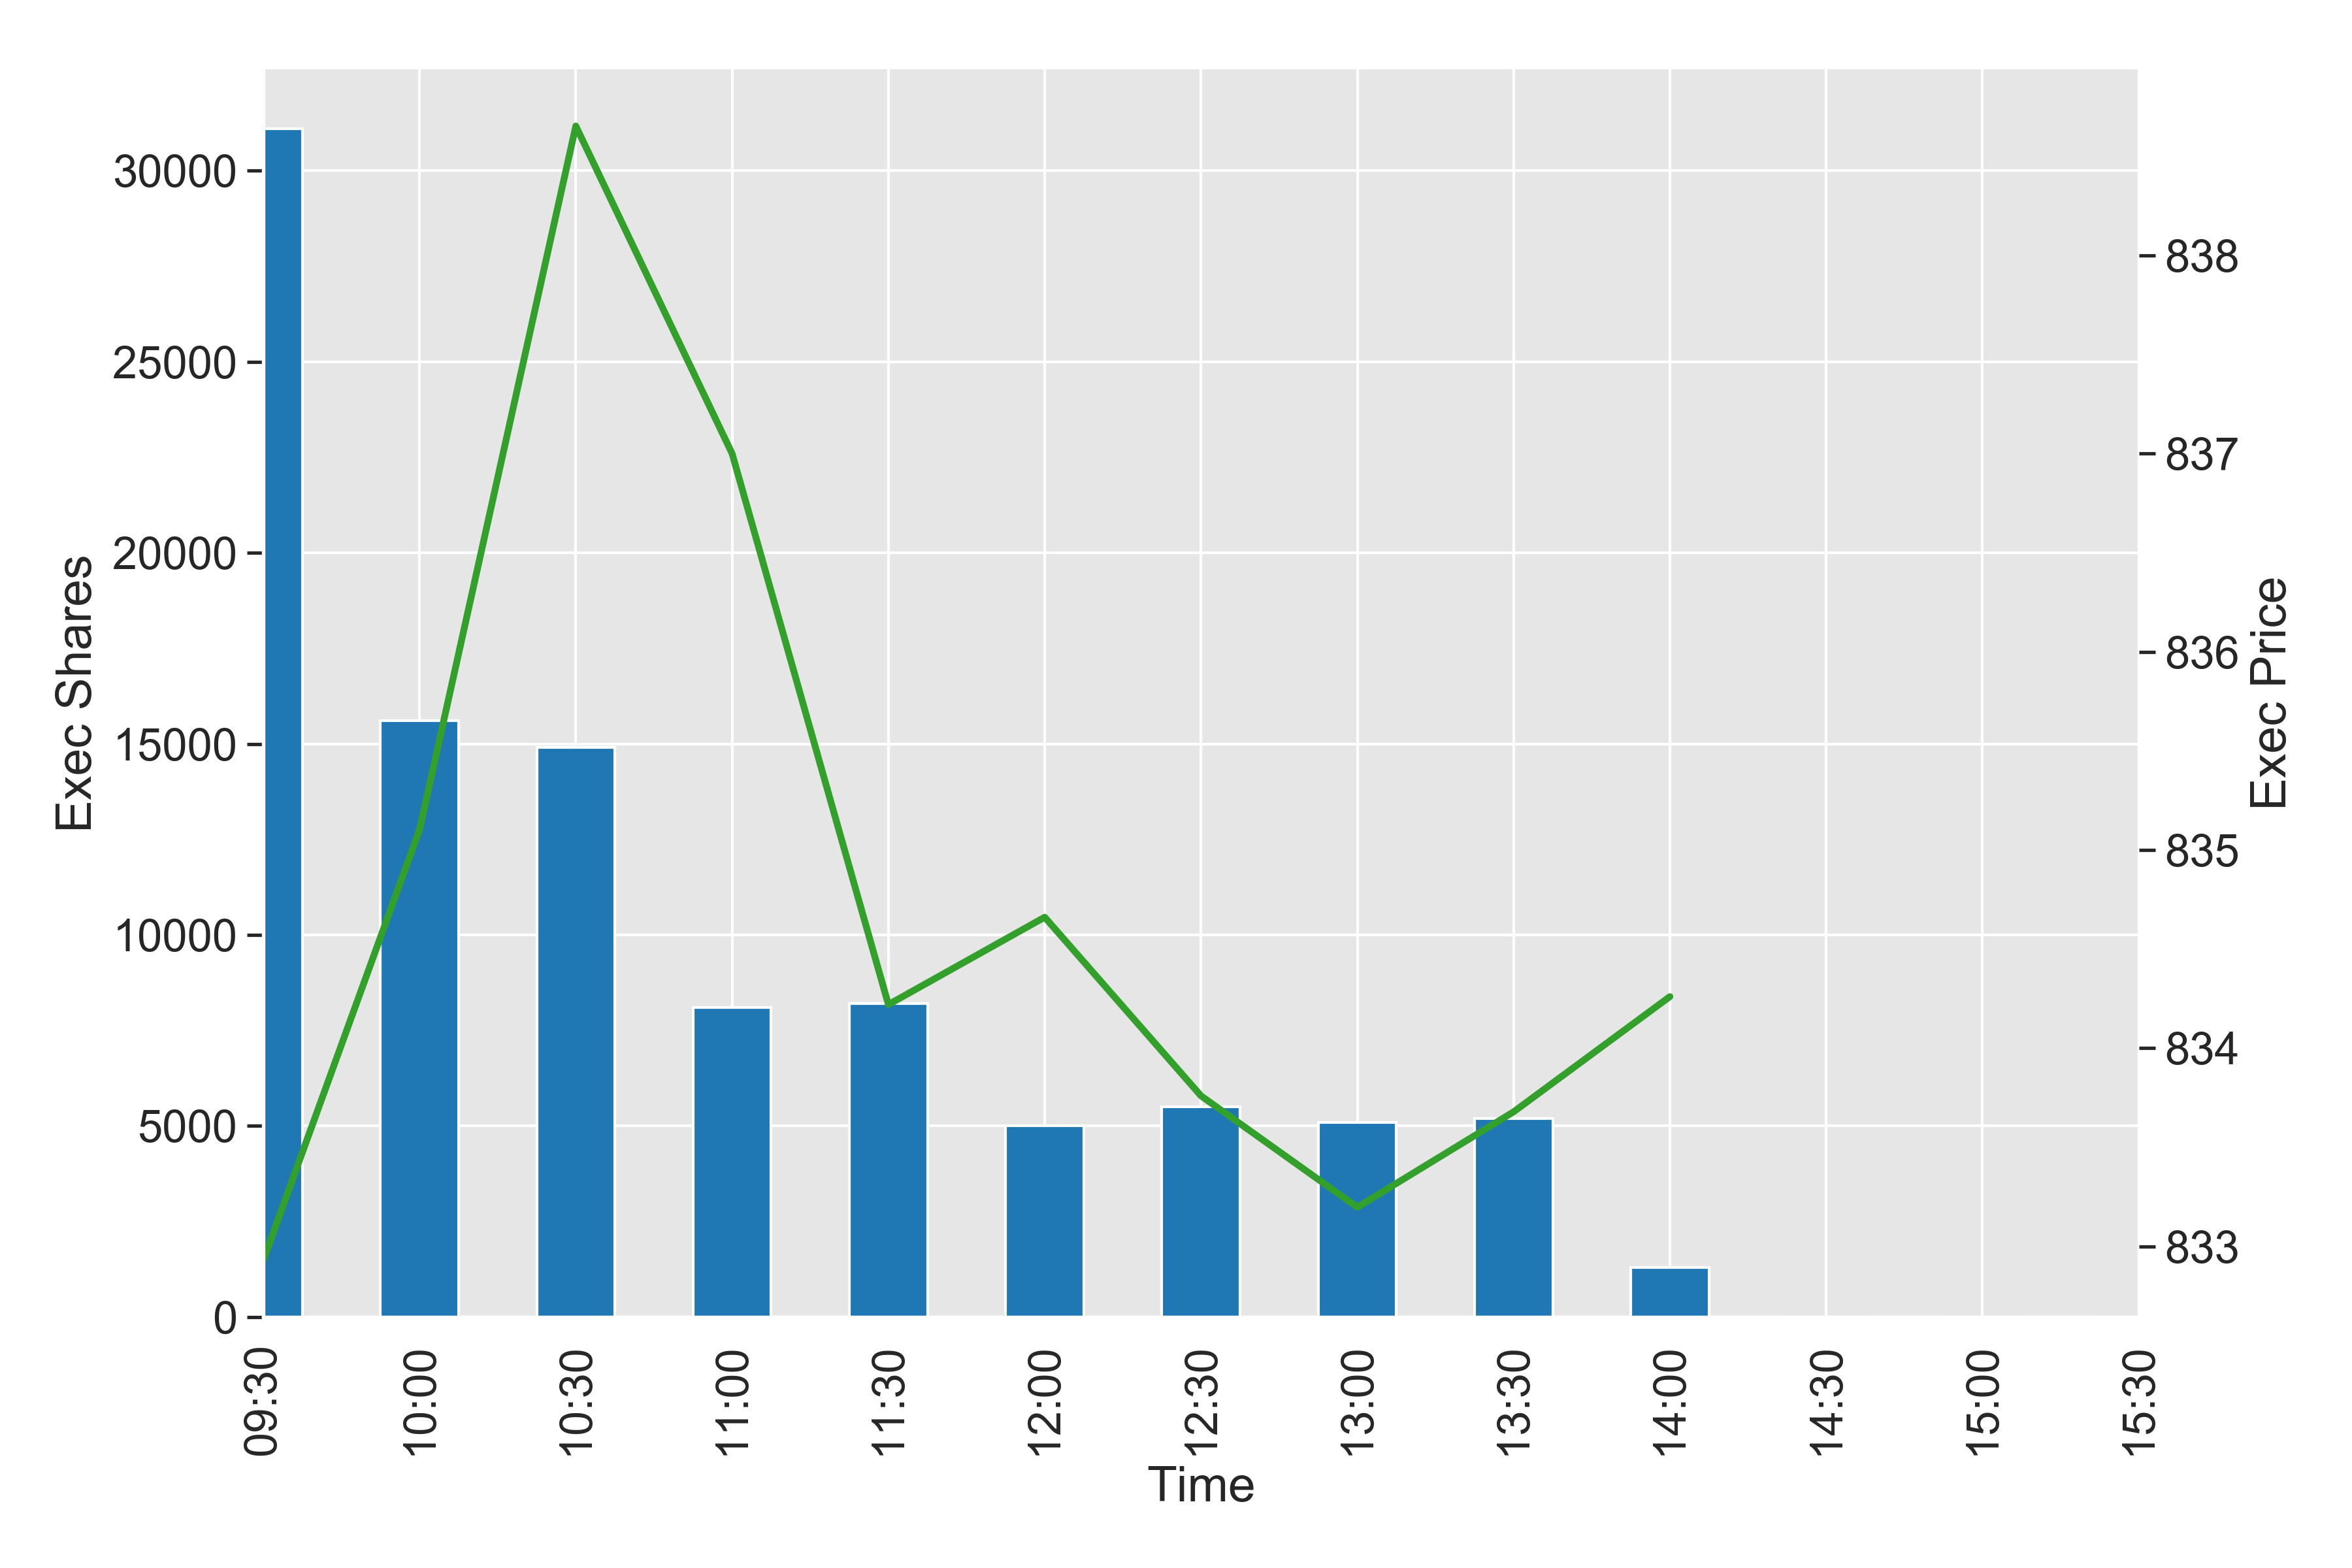
\includegraphics[width=0.75\textwidth]{chapters/chapter_exec_models/figures/pov.png} 
	\caption{Example of 5\% POV Trade for AMZN \label{fig:pov}}
	\end{figure}


\noindent\emph{Close:} \\

Most quantitative strategies leverage close-to-close time series. As a result, some of them favor this price point as a benchmark for their execution strategies. This is also the case for passive indexers whose fund tracking error is computed based on close prices. This clearly places a particular importance to the closing price and thus the desire to minimizing the risk form large negative deviation from that price.


The Close strategy (aka Target Close) was devised to handle this usecase. It's important to understand that in general even Target Close is an IS strategy in the sense that it's after the elusive best price possible. If it wasn't and the ultimate price was unimportant the strategy would be simple: place the whole order as a MOC into the closing auction no matter how big. The close price could be negatively affected by the excess imbalance but the order WILL achieve the close price. So the actual objective is still to get the best price but doing it while avoiding too large of a gamble. If no expectation on price direction is available then the only way to minimize that risk is to trade close to the closing auction as possible. Most strategies attempt to forecast the amount of volume into the close and size the MOC order accordingly to limit the chance of an adverse impact to the closing price and then trade the rest in the latter part of the continuous phase accelerating the trading rate into the close. \\



\noindent\emph{Auxiliary Benchmarks:} \\


On top of these standard primary benchmarks, several additional metrics are used to shed more light on execution performance:

\begin{itemize}
\item \textbf{Completion rate:} while achieving low slippage versus arrival price might be considered as a desirable outcome, if only a fraction of the parent order got executed, the user of the execution strategy is left facing a potentially significant opportunity cost as the expected alpha wasn't fully captured. In order to avoid rewarding strategies that achieve low implementation shortfall just by being extremely passive and stopping trading when prices become unfavorable, most practitioners add a penalty term for the unexecuted portion of the order. There are several approaches to do so, one of the simplest being to apply a slippage to the unexecuted quantity equal to the difference between the arrival price and the close price of the day. 

\item \textbf{Close:} Even if not the central benchmark discussed above the close price being the last accessible price of the day, it is often used to compute the opportunity cost for unexecuted quantity. 
There are different variations of this benchmark, most notably benchmarking execution performance versus the previous close (for strategies that select their target holdings through an overnight process using the latest available close price as an input in their model) or the open price to reflect the fact the previous close is a price point that was not accessible to the strategy.

\item \textbf{Make/Take ratio:} this ratio provides some indication of the execution efficiency. How much of the liquidity was sourced on the passive side of the spread (at the bid or lower for a buy order), versus how much required the algorithm to pay the spread? This metrics highlights the quality of the order placement of the execution strategy though its ability to provide liquidity while achieving its desired trading rate. It is worth noting, however, that more passive fills do not guarantee overall better performance with regard to the primary benchmark. For instance, if a security exhibits strong intraday adverse momentum, a very passive strategy favoring passive fills would result in lower participation rates, hence delaying the total execution and exposing the user to worst prices later in the day. Similarly, highly passive VWAP algorithms do not always have better slippage versus VWAP. As the security price moves away, the algo will progressively fall behind its target schedule, only to catch up to it once hitting the bands controlling the deviation from target, but at a worse price than at the beginning of the period.
One should also ask themselves if a buy child order finally getting filled passively after being re-pegged successively to an increasing bid price represents a better execution than having paid for the spread right at the beginning of the period.\footnote{As throughout this book, the reader is encouraged to remain critical when analyzing performance benchmarks and metrics, and eventually create more sophisticated versions of them to more accurately capture existing trade offs.}

\item \textbf{Mean vs. Variance of performance:} while absolute performance tends to be the main focus of execution benchmarking, a trader might also want to control the level of dispersion around the mean. In practice, traders with large amounts of flow on a daily basis often focus more on the attained mean as their risk of being adversely affected by outliers is somewhat mitigated by the number of orders. Conversely, occasional traders are often willing to accept a slightly less optimal mean performance if it is accompanied by a reduced variance of performance.
\end{itemize}



% Evolution of Execution Strategies
\subsection{Evolution of Execution Strategies}


The section above described the main approach used by the original Algorithms that still account, combined, for most of the trading flow going through execution algos around the globe. These were also the  first strategies to be created. They were conceptually simple but overall quite effective. While over time they evolved in sophistication by using better analytics, order placement, and more nuanced handling of the schedule, the approach to the strategies have small quantitative sophistication.


As the business evolved practitioners where looking for better approaches, something that would have some quantitative underpinning that would move beyond the naive methods of the first algorithms.


We briefly look at how these efforts evolved and the drivers behind the evolution. \\


\noindent\emph{Implementations Shortfall} \\


At the turn of the century things changed with the seminal paper from Almgren and Chriss (2000)~\cite{alm2000} that proposed an approach to ``optimal execution.'' Finally, a more quantitative treatment of the subject, the approach was based on a variational  mean-variance optimization framework similar in spirit with the Markowitz optimal portfolio allocation setup.


We will discuss the more mathematical setup and results in the section around optimal execution academic literature. Here we limit ourselves to the high level results of the approach. The optimal schedule, claim Almgren and Chris (2000), is one that trades-off minimizing impact with the volatility of the overall cost. Like Markovizt the tradeoff between mean and variance is governed by a hyperparmeter $\lambda$ which was meant to incorporate the specific ``risk aversion'' of a particular trader. Since the overall volatility cost depends on the remaining quantity the variance is highest at the beginning of the order and thus the optimal schedule will trade-off more impact cost and thus a higher trading rate to reduce that variance. As the position decreases the risk decreases and thus the optimal schedules reduces its trading rate. The optimal schedule displays a very typical front loaded shaped curve that vanishes to zero at the trading end time.


The approach generated a huge amount of interest in the industry and  brokers increased their investment in quantitatively strong personnel who could understand and implement these strategies leading to the evolution of a new type of quant: the execution quant. Most algorithm providers implemented a version of this algorithm and hailed the arrival of the ultimate solution to the IS problem. 


The incredible popularity of the approach that there were important math-finance problems in trading led to a dramatic increase in the academic community to find better and better approaches to the Optimal Execution problem.\footnote{Since the approach is fundamentally based on the dynamics of market impact this renew interest added  a hugely important side benefit of a significant increase in the research of market impact models} We will discuss the highlights of the evolution of the optimal execution field of study in the next section.


But there was dissent in the troops! Many traders were highly skeptical of the approach. They did not believe that a completely static curve could really be the optimal way to trade a name, with complete disregard of what is happening in the market at a point in time. They believed that a real IS strategy should be dynamic, picking spots,  backing off when prices are not good and take advantage of advantageous prices.  Additionally, the dramatic increase of dark liquidity that promised ability to trade in large positions with zero (limited) impact, challenged the idea of a static schedule to achieve the best price possible. Finally most implementation where problematic because they did not account for the possibility of the order being amended. Because most algos infrastructures, when a parameter is changed, do not maintain any state and they react by creating a brand new parent order. The IS optimization will re-evaluate the strategy and front-loaded again the schedule creating further impact on the stock. For trader that use tight limits this created real havoc.


Some buys side quants were also skeptical. They realized that actually the IS schedule, by being a mean variance trade-off, are actually not providing the best price. The optimization actually trades off some mean cost for a reduction in the standard deviation.  But to large trading operation the mean is really the only thing that matters. They would take additional volatility if the could achieve a better price. So they claimed that their risk aversion was zero. What happens when in this beautiful quantitative model, one goes for zero risk aversion? The the reduction in market impact is the only component and the Almgren-Chris model reduces to\dots  wait for it\dots VWAP! So a whole subset of users shrugged off the revolution and continued to use VWAP as their main approach.


Execution quant struggled to adapt the IS framework to incorporate the feedback. The restrictive mathematical framework made it complex and awkward to evolve. Several providers kept the ideas but abandoned the original formulation, other tried to incorporate some more dynamic approach by moving to a stochastic control framework, other still kept the original formulation fixed and bolted on a set of heuristics.


New academic work expanding on the framework came out with more extreme optimal execution schedules and where largely ignored as unrealistic by practitioners. While the debate is still ongoing and there are a few IS implementations that follow the original framework the whole approach is slowly falling out of favor in favor of a more dynamic set of algos. \\

	\begin{figure}[!ht]
	\centering
	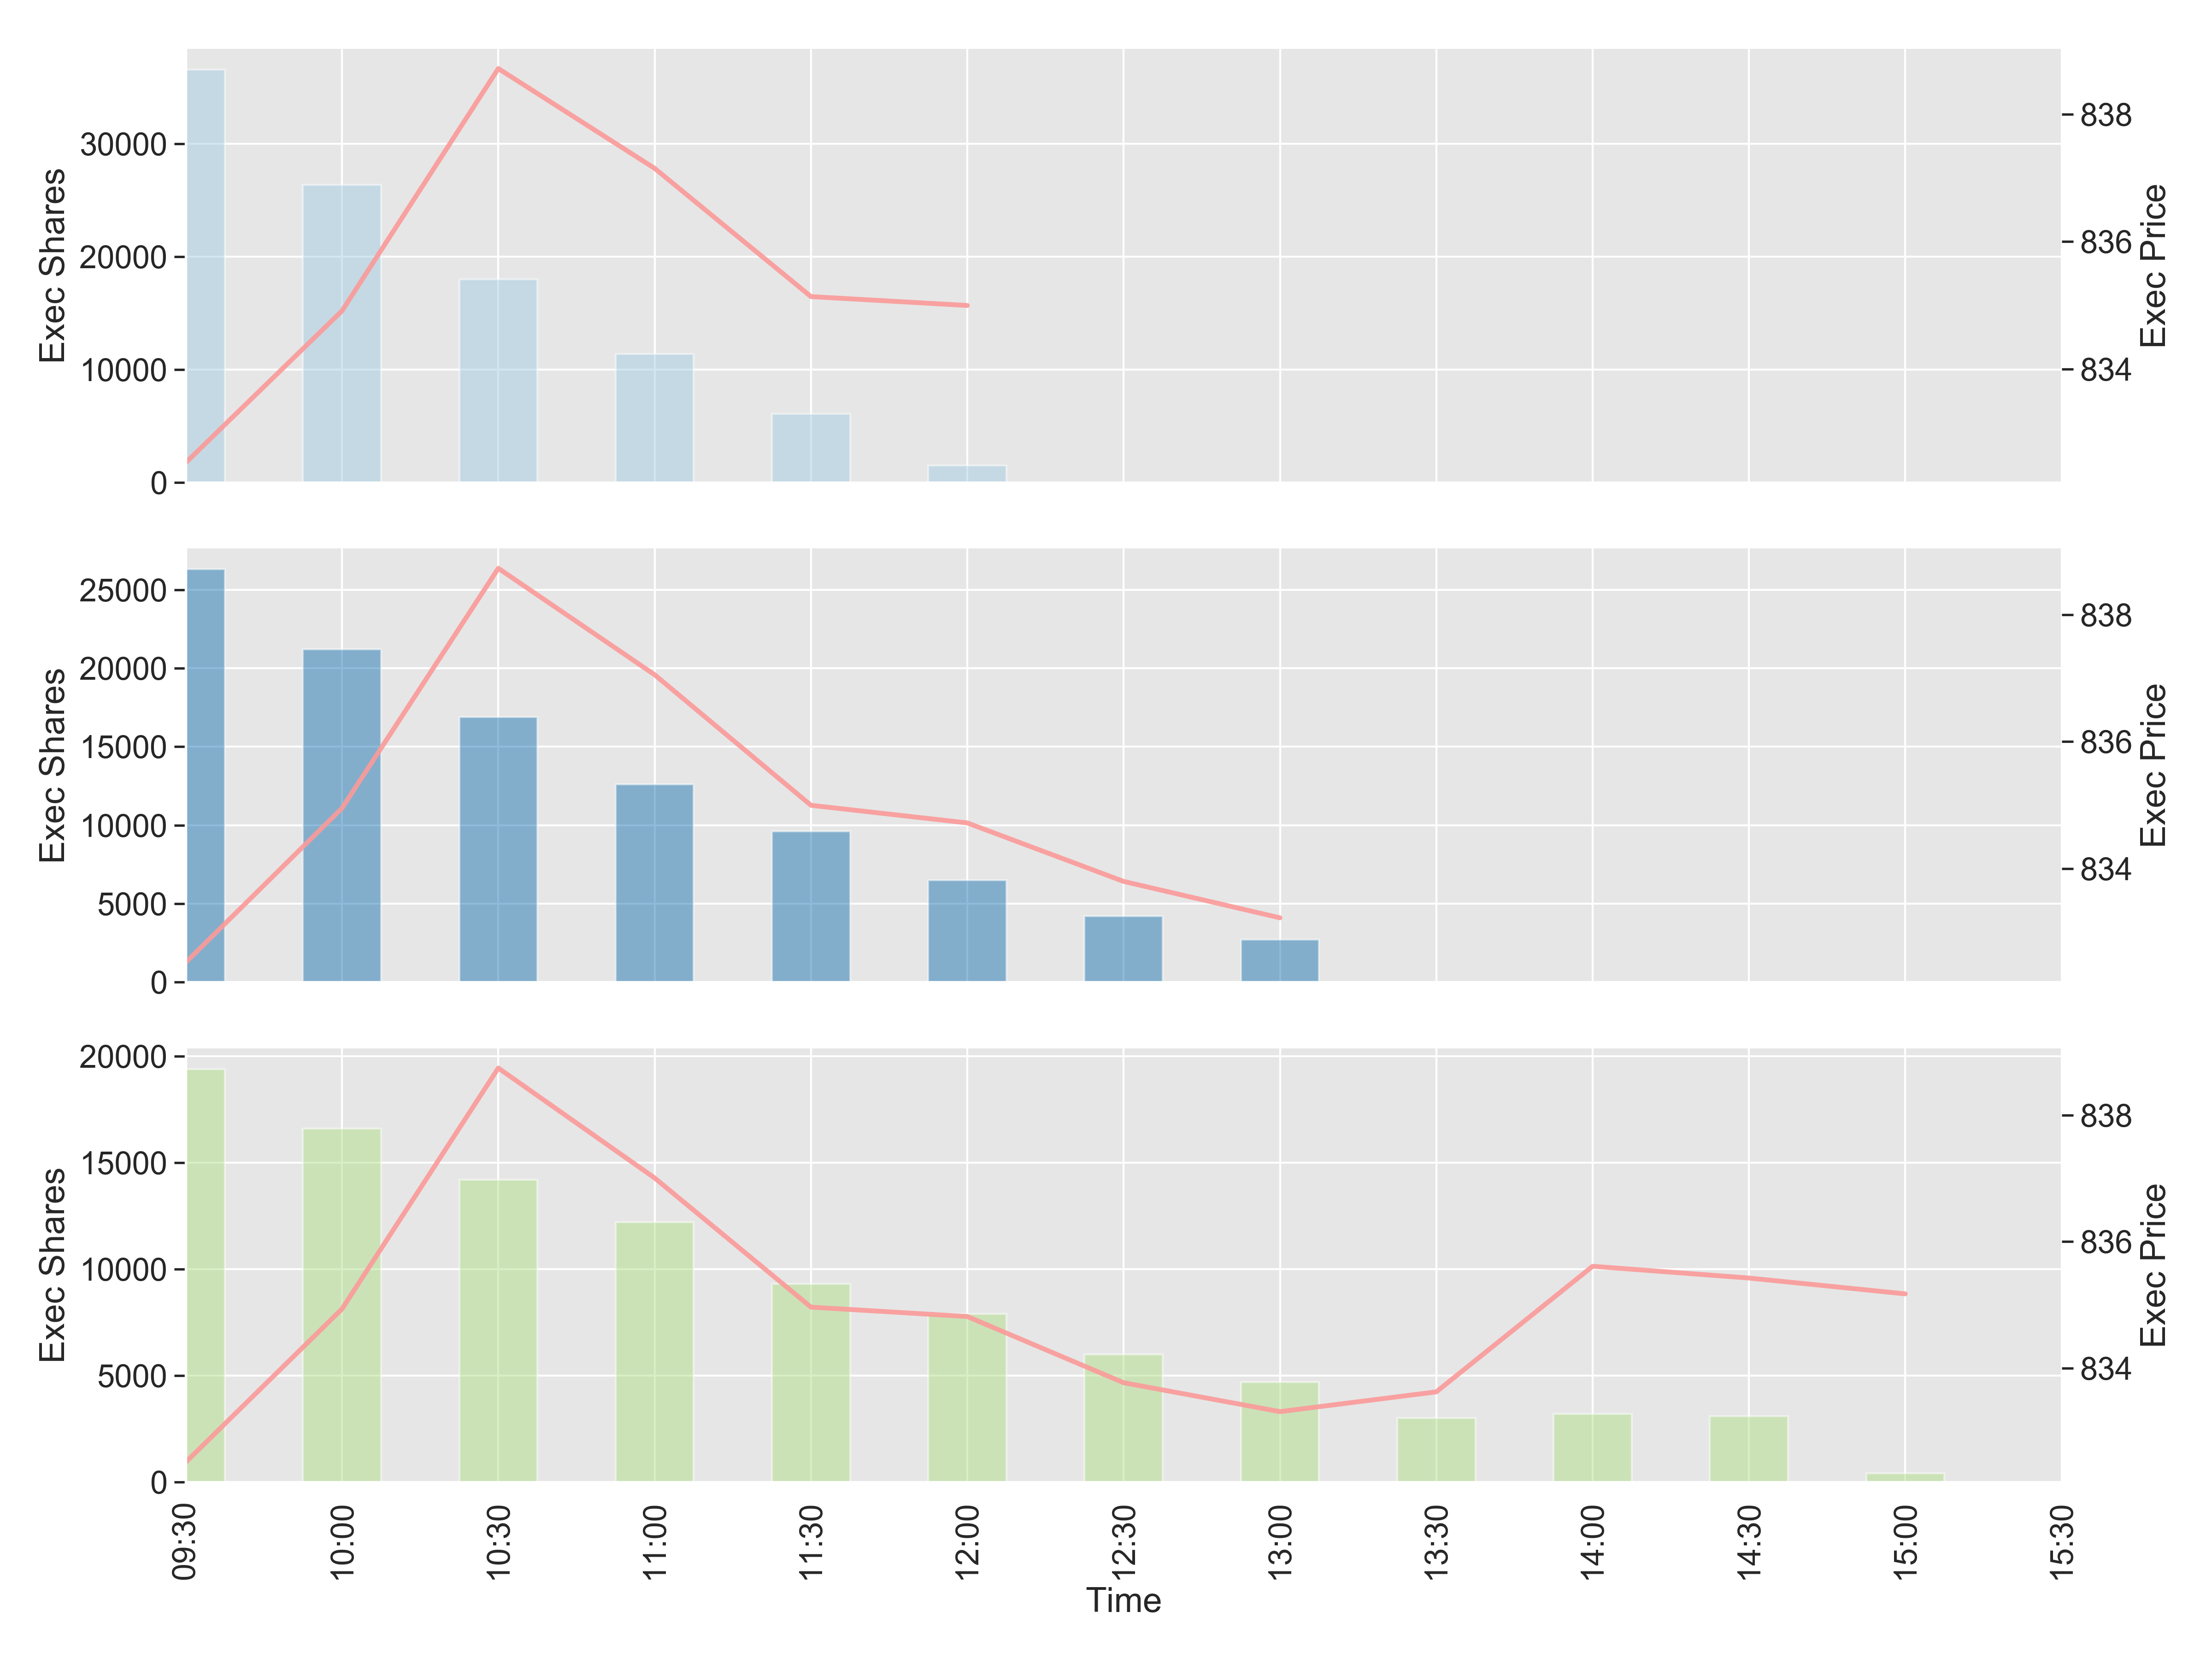
\includegraphics[width=0.75\textwidth]{chapters/chapter_exec_models/figures/is.png} 
	\caption{Almgren \& Chris solution for different ris aversions \label{fig:is}}
	\end{figure}



\noindent\emph{Portfolio IS} \\


One area where the approach took more hold was in the portfolio level space where the risk was actually meaningful and there was a need for a linked execution schedule to avoid a well balanced portfolio from becoming unbalanced and be exposed to market (and other factors) risks. The available implementations provided by brokers are to a large extent still based on the original framework. Very few of them, in the author's opinion, work incredibly well and there are a lot of complexities and shortcomings that still need to be resolved both from the numerical approach and performance (Most implementation leverage QP solvers and to create a flexible implementation for large portfolios that can be optimized in a reasonable time frame requires a lot of tricks and shortcuts) as well as better handling of dark liquidity. \\


\noindent\emph{Liquidity Seeking Algos} \\


The next evolution of algorithms, broadly named Liquidity Seeking, are to some extent a rejection of schedule based approaches that had dominated up until then. This came as a recognition that often schedule have to make sub-optimal decisions in order to purely maintain a schedule and these decision have significant impact on the performance of the strategy. By abandoning the schedule for a completely dynamic approach the hope was that the excess impact due to ``schedule catch-up'' behavior would be reduces.


Liquidity Seeking algos encompass a whole set of approaches and urgencies from very aggressive taking as much liquidity as possible up to a certain maximum limit price, to completely Dark strategies that posted all liquidity in dark pools, to highly opportunistic strategies that would pounce at particular situations in the market such as far-side outsized liquidity (i.e. when the visible quantity at the far size is unusually large)\footnote{Far side outsized liquidity is essentially similar to quote imbalance which, we discussed, points to the price going in the favor of the order. Taking all that liquidity at that price is thus counter-intuitive and there is no evidence that the approach is highly beneficial if not coupled with other metrics}, to everything in between.


The downside of these approaches is that, since there isn't a schedule to follow the behavior can be highly non-deterministic and it implicitly excludes any timing risk component. The order that does not find enough liquidity would remain incomplete possibly to a large extent. That order would then have to be traded the next day. Traders started demanding that the algo at least maintains a minimum participation thus reintroducing an underlying scheduling component. Another issue introduced by the early days overuse of dark liquidity is that it has inherent risk of adverse selection. If the residual of a large order is fully executed at the midpoint, there is a high degree of probability that the price immediately after the trade would be more attractive thus creating a regret. This led some traders to demand that even in the dark the order should be ``paced'' again reintroducing a concept of a schedule.


In the last few years, trading style innovation in the execution space has somewhat tapered off. This slow down in new algorithmic approaches is partly due to the push of many buy side trading desks towards a more predictable and systematic attitude toward strategy and algo providers selection. The so called ``Algo Wheels'' are becoming more and more popular in large buy side institutions as their requirements for demonstrating best-execution require a simplification and an homogenization of trading approaches in order to  efficiently use as much as the sample set to make data driven decisions. 


Competition is as fierce as ever if not more due to recent regulatory changes driven by Europe's MIFID II regulation.  However the focus has mostly be on improving the various underlying components looking for more sophisticated approaches that can further squeeze out performance from existing strategies. To some extent sophisticated traders have started moving away from strategies and more towards more abstract objectives and constrains allowing brokers to pick the best approach to achieve them and engaging with the algo providers with unprecedented openness in their effort to truly minimize their overall trading costs. The benchmarks haven't changed and are still as confusing and elusive however relative performance is relatively (pun intended) easy to measure thus at least workable. This new freedom to experiment and single-mindedness focus on performance is leading to a renewed energy and innovations that could signal a new ``Golden Age'' of electronic trading.



% Execution Algorithms for Multiple Assets
\subsection{Execution Algorithms for Multiple Assets}


The execution of trading entry-exit decisions can be made using the methods described in the earlier section for individual assets. Most investors hold multiple assets in their portfolios and evaluate their investments as a whole rather than in parts. In Section~\ref{sec:port_trad_strat}, we discussed the trading strategies with the focus on rebalancing the portfolios. The criteria used were in the traditional framework of mean-variance efficiency with some constraints on the transaction costs. When it comes to execution, the criteria as noticed from earlier sections is on execution costs and the market impact. We will briefly outline some models presented in the literature for multiple-security portfolios.


Only recently there are efforts made to better understand and model cross-impact of trading an asset on trading of related assets. If a trader is liquidating simultaneously multiple assets as part of the rebalancing effort, we should expect some cross-impact. In the low frequency setting this is studied under `commonality' or `co-movement' as discussion in Chapter~\ref{ch:ch_mvts}. In the high-frequency setting, the problem is harder to study due to short-term market frictions. 



% Multiple Stocks: Microstructure Issues
\subsection{Multiple Stocks: Microstructure Issues}


The execution of trading entry-exit decisions can be made using the methods described in the earlier section for individual assets. Most investors hold multiple assets in their portfolios and evaluate their investments as a whole rather than in parts. In Section~\ref{sec:port_trad_strat}, we discussed the trading strategies with the focus on rebalancing the portfolios. The criteria used were in the traditional framework of mean-variance efficiency with some constraints on the transaction costs. When it comes to execution, the criteria as noticed from earlier sections is on execution costs and the market impact. We will briefly outline some models presented in the literature for multiple-security portfolios.


Only recently there are efforts made to better understand and model cross-impact of trading an asset on trading of related assets. If a trader is liquidating simultaneously multiple assets as part of the rebalancing effort, we should expect some cross-impact. In the low frequency setting this is studied under `commonality' or `co-movement' as discussion in Chapter~\ref{ch:ch_mvts}. In the high-frequency setting, the problem is harder to study due to short-term market frictions. 



% Extending the Algorithms to Other Asset Classes
\subsection{Extending the Algorithms to Other Asset Classes}


While the electronification of trading first took place in the equity space, recent years have seen a significant growth of electronic trading and market making in the fixed income world, opening new opportunities to quantitative trading strategies. We give a brief overview of the characteristics of some of these products. 


\begin{enumerate}
\item[\textbf{(a)}] \textbf{Options:} 

\todo{NOTE: Work in progress, still needs completion}

Historically, equity options markets have presented unique challenges to the successful deployment of sophisticated algorithmic trading strategies. First, options markets are significantly more fragmented than their equities counterparts, not just in space (i.e. across multiple exchanges) but also in terms of instruments. For one equity instrument representing a company (or for one index), there is a grid of available options over multiple maturities and multiple strike prices.  

wikipedia def:
The Options Price Reporting Authority (OPRA) provides, through market data vendors, last sale information and current options quotations from a committee of participant exchanges designated as the Options Price Reporting Authority. OPRA is a national market system plan that governs the process by which options market data are collected from participant exchanges, consolidated, and disseminated.

OPRA disseminates last sale reports and quotes. OPRA also disseminates certain other types of information with respect to the trading of options on the markets of the OPRA Participants, such as the number of options contracts traded, open interest and end of day summaries. \\

message rates: 4Q2018 source \url{https://www.opradata.com/}

Peak Messages Per Second (millions): 19.8

Peak Messages Per 100 Milliseconds (millions): 4.2

Peak Transactions Per Day (billions): 45.9\\

Options participant exchanges in OPRA; 
BOX Exchange
Cboe BZX Options Exchange
Cboe C2 Options Exchange
Cboe EDGX Options Exchange
Cboe Options Exchange
Miami International Securities Exchange
MIAX PEARL
Nasdaq BX
Nasdaq GEMX
Nasdaq ISE
Nasdaq MRX
Nasdaq PHLX
The Nasdaq Stock Market
NYSE American
NYSE Arca \\


Automated options market making strategies were the first ones to be deployed, and we are now witnessing the emergence of execution strategies in the option space. for instance targeting certain volatility levels (instead of price-based benchmarks). Given the natural relationship that exists with the underlying assets, options algorithmic trading strategies also require the implementation of automated delta and gamma hedging execution strategies.


It is also worth noting that most exchanges now support order types such as spreads making multi-leg strategies easier to implement.


\item[\textbf{(b)}] \textbf{Credit Derivatives:} 

When an entity, whether private or public, borrows money, the lender or debt holder bears some default risk until maturity. There is always a risk that the entity will not be able to repay the debt in full or per the agreed terms (coupons, maturity, \dots). Credit derivatives allow debt holders to hedge all or part of that risk, as well as speculators to express their views on the creditworthiness of various entities. 


A credit default swap (CDS) is a derivative contract allowing to buy or sell protection on a single reference entity. The protection buyer pays a fixed, running or upfront, premium in return for the right to receive a payment should the reference entity suffer a credit event. Depending on the CDS contract, an eligible credit event might correspond to a payment default on the debt, a restructuring or a simple credit downgrade of the reference entity. In return for the premium, the writer of the CDS agrees to pay to the buyer (1 $-$ recovery rate) times the notional of the contract upon the realization of an eligible credit event. Here, the recovery rate represents the fraction of the face value of the debt that can be recovered following a credit event.


By entering a default swap, the buyer is essentially purchasing an insurance against the risk of default of a borrower. However, that insurance being paid by the CDS issuer bears counter-party risk (the ability of the issuer to pay the agreed amount in the event of a credit event affecting the borrower). Consequently, the valuation of a CDS depends, among other factors, on the default probability of the borrowing entity over the life of the contract, on the default probability of issuing counter-party, as well as the correlation between them.


The estimated CDS notional outstanding stands above \$10~trillions, after having peaked at about \$62~trillions at the end of 2007 (International Swaps and Derivatives Association (ISDA)~\cite{ISDA}), and north of 1~million trades are recorded per week. In the aftermath of the Global Financial Crisis of 2008, trading liquidity shifted from single name CDS toward CDS Indices, which are essentially baskets of single name CDS. Roughly half of the outstanding notional originates from single reference entity contracts, while most of the other half emanates from credit indices (roughly 130,000~trades per week in 2016).


Over-the-counter (OTC) derivatives markets are considered dealer markets, as they tend to be traded through a network of private dealers who stand ready to provide liquidity in various instruments while maintaining a relatively neutral net risk exposure. This, traditionally, is conducted one on one, off exchanges. However, the introduction of the Dodd-Frank Act of 2010 brought significant transformation to the U.S. swap markets by mandating central clearing for standardized over-the-counter derivatives such as swaps, as well as forcing their execution on a swap execution facility (SEF).\footnote{In Europe, the MiFID II directive adopted by the EU in 2014, with applicability on January 3rd, 2018, also introduces obligations for sufficiently liquid standardized derivatives contracts to be traded only on regulated platforms such as OTFs: Organized Trading Platform.}


The term `swap execution facility' defines a registered ``trading platform in which multiple participants have the ability to execute or trade swaps by accepting bids and offers made by multiple participants'' (Dodd-Frank Act, Section 733~\cite{DoddFrank}). Among the stated goals of mandating swaps execution on SEFs are promoting pre-trade transparency in the swaps market as well as facilitating the real-time publication of trading information such as price and volume to enhance price discovery. As such, the Dodd-Frank Act addressed for swap markets the three main challenges that had historically prevented a significant electronification of trading in fixed income markets: 1) lack of standardized instruments, 2) lack of centralized trading platforms, 3) lack of available transaction data.


SEF usually offer multiple trading protocols giving investors the flexibility to choose the most appropriate trading style for their needs. Existing trading protocols center around either an Order Book-like approach where all markets participants have the ability to execute available bids or offers from multiple participants as well as leave their own limit orders; or a Request-For-Quote (RFQ)-like approach where participants request a single or two-sided market from multiple dealers during a real-time auction.


A variety of credit Indices are fairly liquid and trading on SEFs, in particular U.S. indices (CDX(c)) and European indices (iTraxx(c)). The CDX indices are further broken out by the type of debt covered such as Investment Grade (IG) and High Yield (HY) for the most liquid ones. Due to their liquidity, both CDX IG and CDX HY are examples of credit indices that lends themselves well to electronic market making activities.


However, the CDS Index market presents a certain number of idiosyncrasies compared to equities markets when it comes to market making. While there is an order book available to all participants, most of the volume still gets transacted via RFQ mechanism for which market makers are not always allowed to see the quotes. Consequently, market makers only have partial information regarding the true position of the market when time comes to decide where to place their own orders. Using a a mixture of historical trades and partial real-time information, market makers can reconstruct a theoretical mid price of the market. They can set then the bid and ask quotes at an appropriate distance from that mid price, accounting for the trade-off between their desire to obtain a fill and the risk associated with maintaining their inventory. 


\item[\textbf{(c)}] \textbf{Corporate Bonds}: 

The corporate bond market is also an OTC market where market participants only have access to limited information prior to placing a trade. The main market participants can be categorized as pension funds and insurance companies which tend have longer investment horizons, hedge funds which tend to have more tactical trading allocations, and corporations treasury departments whose objectives and horizons can span a wide spectrum.


Compared to other assets, it is also interesting to note that most of the secondary market transactions happen in the first few months following issuance, and after that a significant portion of the amount of bonds issued is held to maturity. Similarly to other fixed income products, the key challenges for secondary trading of bonds and the electronification of its secondary market have historically been 1) lack of centralized market place, 2) lack of harmonized instrument characteristics and 3) lack of transaction data.


The corporate bonds secondary market remains dominated by one-to-one privately negotiated trades, but electronic platforms allow transacting via similar execution protocols as what traders can use for CDSs: limit order book type of executions as well as request-for-quotes (RFQ) on platforms such as Tradeweb, Bloomberg, MarketAccess and a variety of others.


In the U.S., for instance, under FINRA Rule~6730, Broker-dealer FINRA member firms have the obligation to report transactions in TRACE-eligible securities to the TRACE\footnote{Trade Reporting And Compliance Engine} database as soon as practicable, but no later than within 15~minutes of the Time of Execution. FINRA Rule~6710 defines TRACE-eligible securities as USD denominated debt securities (whether issued by a U.S or foreign private issuer), and USD denominated debt issued or guaranteed by an Agency or Government-Sponsored Enterprise. Foreign sovereign, U.S. Treasuries and money market instruments are specifically excluded from the eligible list. The TRACE database then disseminates price, size,\footnote{The actual size disseminated back to the market is capped to prevent excessive information leakage: for investment-grade corporate bonds and agency debt securities, for any trade greater than \$5~million, the par value is displayed as \$5~MM$+$; for non-investment grade corporate bond, the displayed quantity is capped to \$1~million par value} time stamp and direction of the trade to the public.


While the rules require reporting in no more than 15~minutes, most reporting and public dissemination now happens within seconds or minutes of execution (with the exception of overnight trades being batch-reported the next morning), giving participants some transparency about the current market levels.


The combination of existing venues allowing for click-to-trade or RFQ protocols and trade events information facilitated the expansion of electronic trading for corporate bonds as well. A fifth to a quarter of the investment grade market is now transacted electronically, while on the high yield side, roughly 10\% of the market is traded through RFQs.


Similarly to credit indices, the first challenge for dealers in corporate bond electronic market making is to infer the value of the current ``fair mid'' for the market following each transaction. Given the relatively infrequent updates observations even for bonds that are considered liquid, quantitative techniques employed tend to vary from the ones used in markets with higher frequency data available such as equities. Practitioners rely much more, for instance, on probabilistic state-space models to estimate unobservable data.


This type of approach obviously becomes increasingly more challenging as one moves down the liquidity spectrum. It is not uncommon for illiquid bonds to not trade for months, in which case assessing a fair mid price cannot solely rely on prior transactions. Among possible solutions, modelers can use bonds of other maturities from the same issuers, or bonds from correlated issuers or comparable investment grades. Additionally, more liquid credit derivatives are also a potential sources of information that can be leveraged for better valuations.
\end{enumerate}



% Components of an Execution Strategy
\section{Components of an Execution Strategy}

Regardless of the underlying implementation the approach of and execution strategy can be decomposed in a set of trading concerns that are well understood and to some extent looked at separately. In this section we review these components one by one and provide high level thoughts around modern approaches.



% Scheduler
\subsection{Scheduler}

In electronic execution, the scheduling layer is often described as the macro trader of the strategy, in charge of decisions spanning the whole order duration such as allocating the parent order quantity through the life of the the order. It answers the question: “how much should I trade in each period?”.
This component is aware of the overall trading intention: benchmark, total quantity to transact, risk aversion parameters, constraints (maximum POV, limit price), and order duration. Taking the example of a VWAP algorithm, the scheduler is the component in charge of following the prescribed volume curve between the start and end times provided by the user. In a strategy benchmarked to the arrival price, the scheduler performs an optimization between expected market impact and timing risk (Almgren-Chriss Implementation Shortfall framework). To derive the allocation, most schedulers discretize the trading day in more or less granular bins (generally one to five minutes), each considered a distinct trading interval to be handled by the child order placement module.


The decisions available to the scheduler aim at optimally implementing the end users objectives defined by their stated benchmark. The first decision is which market phases should the algorithm interact with if not specified by the user. For instance, participating in auctions or not. For illiquid names, call auctions can be a significant source of liquidity so participating in them can limit the need for excessive trading in the continuous session. However, trading too much in the open auction - for example - can create an anchoring effect leading to a more permanent market impact price displacement for the remainder of the continuous session, thereby potentially negatively impacting follow-on executions. As often in electronic trading, there are not always absolute solutions, but trade offs.


The scheduler also plays an important role in  implementing liquidity sourcing preferences, such as how much to participate in volatile periods of price discovery when spreads are wide (e.g. in the first few minutes after the market open), or allocating volume between lit and dark venues (where one trades certainty of execution for lower price impact).


Finally, the scheduling layer is also responsible for appropriately handling microstructure features seasonalities. There are well documented intraday volume patterns that can be leveraged to forecast liquidity, volatility and spreads (see Chapter~\ref{chap:ch_trade_data_models}), both on regular days and special days like index rebalances or option expiries. Seasonality can also be witnessed at larger scales: Mondays tend to have more volume, but also more volatility, Asian markets tend to have early morning price action driven by the outcome of the previous market day in the US, etc. All of these can be leveraged by the scheduler to allocate volume more efficiently over time (front load the execution if the market is expected to move unfavorably, or back load it in case of expected favorable move) and across liquidity sources (lit or dark markets). 


It is worth noting that when decomposing execution slippage, the largest contribution can generally be attributed to the scheduling layer, and can range from a few to double digits basis points. Consequently scheduling remains an area of active research for both academia and practitioners.



% Order Placement
\subsection{Order Placement}


The order placement layer sits downstream from the scheduling layer and can be seen as the micro trader of the strategy, in charge of decisions spanning the upcoming few seconds or minutes of trading. While it is generally unaware of the overall trading intention received by the scheduler, it is responsible for implementing locally its decisions. As such, the micro trader answers the question, ``at what price should I trade the quantity allocated for the upcoming period in order to complete and obtain the best possible price?.''


By nature, this component leverages techniques that are very similar to the ones employed by market making strategies, aiming to capture passive liquidity while avoiding adverse selection. The order placement component is also responsible for the decision to cross the spread, either to capture an opportunity, or to attain a desired participation rate if the liquidity sourced on the passive side is not sufficient. Consequently, it relies heavily on microstructure models to take advantage of short-term order book price movements. Among the most commonly used signals for order placement, we can mention:


\begin{itemize}
\item \textbf{Order book imbalance:} When the displayed quantity in the lit order book is significantly imbalanced between the bid and ask sides, it tends to predict an impending up tick or down tick (e.g. larger quantities at the bid are indicative of excess buyers, likely resulting in an up tick as competition for queue position increases).

\item \textbf{Trade imbalance:} This signal aggregates market executions over a period of time and attributes a sign to each of the trades recorded on the tape (essentially, prints happening above the prevailing midpoint are considered buy-initiated, the ones happening below are considered sell-initiated, and the ones happening at the mid are generally given the same sign as the trade immediately preceding). The ratio between buy and sell initiated trades can also be used as a predictor of the direction of the next order book move.

\item \textbf{Weighted midpoint time series:} For names with wider spreads and dense order books, it is possible to construct a time series of the quoted-size weighted average of the bid and ask representing the theoretical fair midpoint price, which is more precise than the effective midpoint only leveraging the quotes, and can be used to infer the trajectory of the order book.

\item \textbf{Trading and cancellation rates:} Using Level~III market data feed, it is possible to track the activity in the order book precisely and track order cancellations. Increases in cancellation rates are indicative of subsequent changes in the order book. 
\end{itemize}


While the examples above are simplistic in nature, the limit order placement module is a component where a lot of quantitative sophistication can be deployed given the complexity and high dimensionality of both the state space and action space. In particular, the state/action nature of the problem makes it well suited to modern techniques like reinforcement learning. 


The output of the order placement module can be modeled as an array of price levels and associated quantity such as [ [18.85 ; 600], [18.84 ; 400], [18.81 ; 200] ] that is then passed on to the order router for execution or quoting on the market.



% Order Routing
\subsection{Order Routing}

The order routing layer sits downstream from the order placement layer and is generally a standalone component - known as the Smart Order Router (SOR) - in charge of the highest frequency decisions (of the order of microseconds to milliseconds). While it is also generally unaware of the overall trading intention received by the scheduler, it is responsible for implementing the decisions of the order placement module. As such, the SOR answers the question ``to which exchange(s) should I route the child order in order to maximize my probability of getting a fill at or better than the desired price?.'' This component is of particular importance in fragmented markets, and might be absent in execution strategies interacted with single markets (EM Equities, Futures, etc.)


Lit and Dark order routing present different challenges. While lit executions and order books are public and can be observed in market data feeds, dark order books are invisible and dark executions tend to be reported in aggregate (for instance, under a single condition code), thus making attribution of actual execution venue more challenging. For instance, if solely observed from market data, dark executions in the US cannot be directly attributed one of the numerous non-displayed venues. However, if observed from the point of view of an executing entity (through execution fills received), one is in possession of sensored observations of the available---otherwise invisible---liquidity (I.e. When receiving a fill for X shares one knows there was at least X shares available to trade on the other side in this particular venue). 


The SOR implements both the aggressive and passive child order submissions, accounting for their respective goals:

\begin{itemize}
\item \textbf{Aggressive Orders:} The order placement can generate passive child orders for two main reasons. First, the existence of a trading signal indicating an opportunity to capture advantageous liquidity (being due to its size or price), and second, the need to catch-up to a desired target execution schedule (for instance after hitting the lower band surrounding the schedule due to insufficient passive fills). In the first case, the opportunity being short lived, the focus in on speed of execution. Given the prevalence of high frequency market makers providing liquidity across multiple exchanges, if a trader want to extract as much liquidity as possible, she needs to prevent liquidity fading.\footnote{Fading occurs when trying to access liquidity at multiple exchanges and, following the execution of a first child order at one of the exchanges other market participants cancel their displayed orders before the other child orders could reach the respective exchanges where the liquidity was previously displayed. This is possible due to the latency that exists when sending orders to multiple, physically distant, exchanges} Depending on the desired size to trade with respect to the aggregate available liquidity at the far touch, the SOR might decide to route its child orders by descending order of liquidity available, or by descending order of expected latency to reach the various exchange - sending first the order to the farthest exchange and timing subsequent submissions so that all child orders hit all exchanges at virtually the same time. 


In the second case, the objective of the aggressive order is just to catch-up to a prescribed schedule with a low-frequency granularity (of the order of minutes), so the routing is not particularly time sensitive. This allows the SOR to first search for opportunities for price improvement, for instance by sending orders at midpoint to a series of dark pools, prior to employing similar techniques as above to fill the remainder of the quantity at the far touch.


\item \textbf{Passive Orders:} When submitting passive orders, the objective is optimize queue position in order to maximize the probability of obtaining a fill\footnote{The SOR can be either cost-agnostic and favor fill rates and time to fill, or cost-aware and try to maximize rebates in markets that have a maker-taker pricing model. This would, obviously, result in different routing strategies.} before the market moves away, while competing with the other liquidity providers. From a modeling standpoint, the SOR objective functions for passive orders can be summarized as:
    \begin{itemize}
        \item Lit Order Routing logic: given $X$ shares to execute, $[n_1, n_2, \ldots, n_Y]$ shares displayed on the book of lit venues $[1, 2, \ldots, Y]$ and some expected trading rates at each venue, what is the combination of shares sent to different venues that maximizes the fill probability and minimizes the time to fill?
        \item Dark Order Routing logic: Given $X$ shares to execute and $Y$ available venues with unknown available liquidity, what is the combination of shares sent to different venues that maximizes the fill probability and minimizes the time to fill?
    \end{itemize}
\end{itemize}



% Review of academic treatment of Execution Strategies
\section{Review of academic treatment of Execution Strategies}


While algorithmic trading techniques are useful in both low and high frequency settings, their importance has become more pronounced in the age of electronic trading because of the speed in execution and the necessity for efficient matching of demand and supply sides in the limit order book. Added to this is that modern equity markets where order submission and cancellations are automated and are also highly fragmented with dozens of exchanges and about forty alternative trading systems where investors can choose to trade. The trading algorithms also differ over various types of market participants, but all of them have common objectives, that is to optimize dynamically where, how often and at what price to trade. The algorithms have small reaction times to changing liquidity and price. Typically, the execution has been broadly classified into the following layers.
	\begin{itemize}
	\item \textbf{Macro Level:} Given a meta-order (parent trade) translate the objective function of a strategy into a trading schedule; when the algorithm should trade, in what size (child order), for how long and the spread of trading.
	
	\item \textbf{Micro Level:} Given a slice (child order) of the meta-order to trade, this layer of algorithm decides whether to place it as a market or as a  limit order and at what price level.
	
	\item \textbf{Smart Order Router:} For a given order (quantity and price level) to which venue should the order be sent. This part covers the so called space dimension.
	\end{itemize}


In this chapter, we discuss these and other execution issues in the high frequency trading context. Generally the objectives of equity trading are to minimize the probability of making errors---minimizing the trading impact and avoiding adverse selection. In order to achieve high completion rates, the trading should operate with speed and necessary risk control. It has to be noted that the average trade size has come down over time; thus the parent orders are increasingly decimated and are sent to the exchanges as small child orders. Handling this with large parent order sizes with the focus on short-term alphas requires a great deal of trade timing insights.  


The execution agencies engage in providing pre-trade advice and post-trade reporting. The pre-trade advice include the estimation of market impact cost covered in Chapter~\ref{chap:ch_mi_models} and the post-trade reporting is useful for evaluating how well the agency's execution algorithm has performed as compared to some benchmarks. These include the fill rate, the fill composition (passive values aggressive covering the spread) and the evaluation measures such as the magnitude of price revision against the order after the trading ends. Different clients are likely to put different emphasis on these measures. 


These algorithms have been generated over time and they depend on how the complexity in trading has grown. In the first generation algorithms focus on trading at fixed rate over a time-aggregated interval, trading at a fixed participation rate and trading such that the average execution price is closer to market volume-weighted average price. The second generation algorithms focus on market impact and risk. The methods here are formalized similar to Markowitz's portfolio theory. Increasing risk aversion generally leads to shorter execution with higher market impact. As more trades occur near the market close, risk averse clients may trade entirely at the closing auction. Finally, the third generation algorithms closely track the state of the limit order book and market data and are adaptive. The optimal decision such as updating the limit price, crossing the spread, cancellation of orders result from stochastic control formulation. The basic data used in these algorithms follow from microstructure signals covered in Chapter~\ref{chap:ch_trade_data_models}. 



% Execution Algorithms: Some Preliminaries
\subsection{Execution Algorithms: Some Preliminaries}


The primary goal of most of the execution algorithms is to minimize the transaction costs which are broadly divided into direct costs and into indirect costs. The direct costs such as commissions, taxes etc are easy to measure and they primarily depend on quantity of trading. The indirect costs such as market impact and opportunity costs are hard to measure and depend upon trading strategies. Because many mutual fund and hedge fund companies engage in portfolio rebalancing periodically, they trade a large block of shares in a fixed duration. There is a trade-off between trading a large market order that is likely to affect the price adversely and splitting the parent order into many child orders and let the market recover after each trade. The modeling elements generally involve representing the permanent impact of a parent order and the temporary impact of trading a child order when the price normally returns back to equilibrium, short time after the trade, drift in price (alpha) and the volatility of the stock. The optimizing function balances the cost-loss in revenue due to price impact and the risk-uncertainty due to volatility of the underlying stock. If the trade occurs fast, we incur high cost and low risk but if the trade occurs slowly, we incur low cost and high risk.


The execution algorithms are generally evaluated through some benchmark prices. Some key quantities are:
	\begin{enumerate}[--]
	\item Arrival price, that is the market mid-quote at the start of parent order execution at $t=0$, $p_0$.
	\item Volume weighted average market price over the period of execution, $t \in (0,T)$, $p_{\text{VWAP}}= \sum_{i=1}^N V_ip_i/V$. \\ \\
	If the parent order of size, $X$ is split into `$n$' child orders with size, $x_k$, $k=1,\ldots,n$, then
	\item Volume weighted average price of the parent order's execution, $p_{\text{exec}}= \sum_{i=1}^n x_ip_i/X$. 
	\end{enumerate}
	
Two other related quantities that the traders examine in their evaluation strategies are:
	\begin{enumerate}[--]
	\item Slippage: $s= p_{\text{bench}} - p_{\text{exec}}$
	\item Market Impact: $p_0 - p_{\text{VWAP}}$
	\end{enumerate}
The execution cost is taken to be the slippage and the execution risk is its standard deviation. 


The influential paper by Kyle (1985)~\cite{kyle1985} argues that traders split the parent order to hide private information. The splitting of the order and how they are sent to the market, the strategies depend on the evolution of the stock price. These are broadly classified into static, one determined in advance of trading and into dynamic, one that depends on the state of the market. The static strategy under some conditions can also be dynamically optimal. Few commonly used criteria for allocation strategies are:
	\[
	\begin{split}
	&\text{VWAP: } x_k= X \cdot \dfrac{V_k}{V} \\
	&\text{Implementation Shortfall: Minimize } E(s) + \lambda \var(s) \\
	&\text{Percentage of Volume: Minimize } \left( \dfrac{\text{Volume}_{\text{exec}}(x_k)}{\text{Volume}_{\text{market}}(v_k)} - v_{\text{target}} \right).
	\end{split}
	\]
These strategies as stated are static and they are based on a priori models for the evolution of price and volume traded over different times of the day. 


We present below select results in this area. The quantities that the trader can determine are the number of child orders $(n)$ and their sizes $(x_k)$ and the duration for the parent order trading $(T)$. The relevance of this problem to the practitioners is discussed in Chan and Lakonishok (1997)~\cite{lakon} and Keim and Madhavan (1997)~\cite{madhavan}. Bestimas and Lo (1998)~\cite{berlo} develop a model that suggests splitting the parent order to reduce the average trading costs. Almgren and Chriss (2000)~\cite{alm2000} split the parent order to minimize the mean-variance of trading costs similar to Markowitz's portfolio theorem. Some recent works on this topic are also briefly mentioned but, describe in some detail in the following sections.



% First Generation Algorithms
\subsection{First Generation Algorithms \label{sec:first_gen}}


The performance of traders is evaluated by how they execute the orders in comparison to volume weighted average price (VWAP), because it is generally considered to be closer to how a passive trader would trade. Madhavan (2002)~\cite{mad_a02} warns that the uncritical use of VWAP are a benchmark can promote non-optimal trading behavior. As noted in the last section, other alternatives to VWAP as possible. The choice of a benchmark will obviously affect the placement strategies by the traders. Using daily VWAP as a benchmark leads to trades spread over the day and thus passive trading can significantly affect alpha. The pre-trade benchmarks such as the arrival price ignore the short-term trends in prices. The post-trade benchmarks are sensitive to order flows towards the end of the day and thus have higher price impact. The VWAP strategy can be automated so that order submissions can follow historical volume pattern during the course of the day with finer time grids. This practical approach is expounded in this section.


We will follow the formulation of the optimization problem as given in Busseti and Boyd (2015)~\cite{busseti_boyd}. With $X$, the total number of shares to be traded over the time horizon, $(0,T)$ in `$n$' discrete time intervals, the problem is to decide how to divide the parent order $X$ into child orders $x_1, \ldots, x_n$ so that the executed average price $p_{\text{exec}}$ is closer to $p_{\text{VWAP}}$. It is assumed that the price, $p_t$, is a random walk and thus the return is white noise. It is assumed that the trading algorithm mixes optimally market and limit orders. Defining the cost of trade in time interval $t$ as $x_t \hat{p}_t$, where $\hat{p}_t$ is the effective price that depends on the instantaneous transaction costs such as bid-ask spread with `$s_t$' as the fractional bid-ask spread with a certain participation rate $x_t/v_t$, it can be shown that the effective price is
	\begin{equation}
	\hat{p}_t= p_t \left(1 - \dfrac{s_t}{2} + \alpha \, \dfrac{s_t}{2} \cdot \dfrac{x_t}{v_t} \right),
	\end{equation}
which gives in the end quadratic transaction costs which is a reasonable approximation as seen from Chapter~\ref{chap:ch_trade_data_models}. Here `$\alpha$' is taken to be proportionally factor of market orders to total orders. Defining the proportional ratio
	\begin{equation}
	s= \dfrac{X p_{\text{VWAP}} - \sum x_t \hat{p}_t}{X p_{\text{VWAP}}}
	\end{equation}
as slippage, where the numerator is the cash flow to the broker, the optimizing function is
	\begin{equation} \label{eq:opt_function}
	E(s) + \lambda \var(s).
	\end{equation}
Here `$\lambda$' is the risk-aversion parameter. It has to be kept in mind that the quantities $p_t$ and $v_t$ are random variables and the decision variable is `$x_t$'. Note with some approximation, $p_t \sim p_{t-1} \sim p_{\text{VWAP}}$ and with applying the law of iterated expectation, the optimization in \eqref{eq:opt_function} simplifies to
	\begin{equation}
	\min_{x_t} \sum_{t=1}^n \left[ \dfrac{s_t}{2x} (\alpha x_t^2 k_t - x_t) + \lambda \sigma_t^2 \left( \left( \sum_{r=1}^t u_r/X \right)^2 - 2 M_t \sum_{r=1}^{t-1} u_t \right) \right]
	\end{equation}
with constraints $x_t \geq 0$ and $\sum_{t=1}^n x_t = X$. Here the quantities $M_t= E \left[ \sum_{r=1}^{t-1} v_t/v\right]$ and $k_t= E[\frac{1}{v_t}]$ refer to market intra-day volume distribution. Assuming that the spread is a constant which is generally true for actively traded stocks, the optimal static solution can be shown to be equal to:
	\begin{equation} \label{eq:optimal_result_xt}
	x_t^*= X E\left(\dfrac{v_t}{v}\right), \enskip\enskip t=1,\ldots,n.
	\end{equation}
From the above discussion, it is clear that forecasting both the intra-day distribution of volume, $v_t$, and the total volume for the day, $v$, is essential for achieving optimal results. The optimal result in \eqref{eq:optimal_result_xt} can be obtained also with slippage as defined in the previous section. \\


\noindent\textbf{Bertsimas and Lo Model:} The basis of the model discussed here is that trading affects not only the current prices but also the price dynamics that affect the future trading costs. Thus the problem involves dynamic optimization but the solution turns out to be static. Assume that an investor wants to sell a parent order of $X$-shares in $(0,T)$, where $T$ is arbitrary, and let $x_k$ be the number of shares sold (child orders) with the realized price, $\widetilde{p}_k$. The cost of trading, also know as slippage is
	\begin{equation} \label{eqn:x7}
	s= Xp_0 - \sum_{k=1}^n x_k\widetilde{p}_k,
	\end{equation}
where $p_0$ is the arrival price. The model proposed in Bertsimas and Lo (1998)~\cite{berlo} can be stated as
	\begin{equation} \label{eqn:xk7}
	\min_{x_k} E_1 \left[\sum_{k=1}^n x_kp_k\right] \text{ such that }\sum_{k=1}^n x_k=X.
	\end{equation}
The criteria in \eqref{eqn:xk7} call for determining the sizes of child orders a priori. To solve \eqref{eqn:xk7}, the model for price, where the price impact and price dynamics are separated, is taken to be,
	\begin{equation} \label{eqn:pk7}
	p_k = p_{k-1} - \theta x_k + \varepsilon_k,
	\end{equation}
where $\theta > 0$ representing the price impact and when $\theta = 0$, the model is simply a random walk model discussed in Chapter~\ref{ch:ch_uvts}. Under \eqref{eqn:pk7} the best strategy for splitting the parent order, $X$, is shown to be
	\begin{equation} \label{eqn:equals}
	x_1^* = x_2^* = \cdots = x_n^* = \frac{X}{n},
	\end{equation}
the equal split. What the trader needs to decide a priori is the number of splits, $n$. The allocation strategy in \eqref{eqn:equals} is termed as the time weighted average prices (TWAP) strategy in industry. 


The dynamic programming solution to \eqref{eqn:xk7} via the so called Bellmann equations turns out to be elegant and simple because the price impact $(\theta x_k)$ does not depend upon the prevailing price $(p_{k-1})$ nor on the size of the unexecuted order $(X - \sum_{j=1}^{k-1} x_j)$. The indirect assumptions here are that the volume curve is even over different times of the day and the volatility profile is flat. Bestimas and Lo (1998)~\cite{berlo} also consider extensions of the model \eqref{eqn:pk7}, where a serially correlated state variable such as market condition (S\&P 500) is added. In this case it is shown that the best execution strategy at any point is a function of the state variable and the remaining unexecuted size. 


As a point of comparison to the equal allocation strategy observe that VWAP-strategy is similar in the sense that is does not also depend explicitly on any price movement. Simply the allocation is made in \eqref{eq:optimal_result_xt} can be intuitively justified as resulting from $\frac{x_k}{X}= \frac{V_k}{V}$. If the traders are restricted to only `$n$' time intervals, it is important to have a good forecast for the quantities, $V_k$ and thus, $V$, the total volume for the day. 



% Second Generation Algorithms
\subsection{Second Generation Algorithms \label{subsec:almchrmodel}}


\noindent\textbf{Almgren and Chriss Model:} The seminal paper by Almgren and Chriss (2000)~\cite{alm2000} and Almgren (2003)~\cite{almgren2003} consider the same problem taking into account the stock characteristics such as volatility via the mean-variance formulation of minimizing execution costs. This formulation treats the execution as a tradeoff between risk and cost; the faster the execution, higher the cost but lower the risk. The objective again is to liquidate, $X$ units before time `$T$' at minimum cost, in time steps, $t_k = k \tau$ for $k = 0,1,\ldots, n$ where $\tau = T/n$ is the average length of interval between successive child order submission times. If $X_k$ is the number of units held at $t_k$, the goal is to decide on the trading trajectory, $X_0, X_1, \ldots, X_n$ with $X_0=X$ and $X_n=0$. The number of units liquidated $x_k$ between $t_{k-1}$ and $t_k$ is called the trading schedule, with $x_k = X_{k-1} - X_k$. The trading strategy requires determining `$x_k$' in terms of information available at $t_{k-1}$. The static strategies determine the trading schedule in advance of starting trade time, $t_0$ and the dynamic strategies depend on information available up to $t_{k-1}$. Almgren and Chriss (2000)~\cite{alm2000} find trading trajectories that minimize $E(s)+\lambda \Var(s)$ for various values of $\lambda$.


The model for price impact is same as in \eqref{eqn:pk7} but stated as
	\begin{equation} \label{eqn:bigpk}
	p_k= p_{k-1} - (\tau\theta)\dfrac{x_k}{\tau} + \sigma \tau^{1/2}\varepsilon_k,
	\end{equation}
where $v_k = x_k / \tau$ is the average rate of trading in $[t_{k-1}, t_k]$ and $\varepsilon_k$ are independent with mean zero and unit variance and `$\sigma$' is the volatility of the stock. The temporary impact represented by price per share received for sale in $[t_{k-1}, t_k]$ is
	\begin{equation} \label{eqn:pdouble}
	\begin{split}
	\widetilde{p}_k &= p_{k-1} - \eta\left( \dfrac{x_k}{\tau} \right) \\
			&= p_{k-1} - c \sgn(x_k) + \frac{\eta}{\tau} \cdot x_k,
	\end{split}
	\end{equation}
where $c$ can be taken to be fixed cost of selling which is the sum of mid-spread and fees. The temporary impact component is not present in the next period. Note \eqref{eqn:bigpk} can be written as
	\begin{equation} \label{eqn:morepk}
	p_k = p_0 + \sigma\tau^{\frac{1}{2}}\sum_{j=1}^k\varepsilon_j - \theta(X - X_k),
	\end{equation}
and thus the shortfall
	\begin{equation} \label{eqn:longxeq}
	s = Xp_0 - \sum_{k=1}^N x_k\widetilde{p}_k = \sum_{k=1}^N \left(\frac{x_k}{\tau}\right) \eta - \sum_{k=1}^N \,[\sigma\tau^{1/2}\varepsilon_k - \theta x_k]X_k
	\end{equation}
is a function of the market volatility and the trade schedule, `$x_k$'. It captures the difference between the initial book value and the weighted average of realized prices. From \eqref{eqn:longxeq}, it follows that
	\begin{equation} \label{eqn:evardouble}
	\begin{split}
	E(s) &=  \theta\sum_{k=1}^N x_k X_k + \eta \sum_{k=1}^N \frac{x_k}{\tau} \\
	\var(s) &= \sigma^2 \sum_{k=1}^N \tau X_{k}^2\cdot
	\end{split}
	\end{equation}
If the trajectory is to sell at a constant rate, $x_k = \frac{X}{n}$ and $X_k = (n - k) \frac{X}{n}$, $k = 1, \ldots, N$,
	\begin{equation} \label{eqn:secondevardouble}
	\begin{split}
	E(s)&= \frac{1}{2}\, \theta\, X^2 + \varepsilon X + \left(\eta - \frac{1}{2} \theta \tau \right) \frac{X^2}{T} \\
	\var(s)&= \frac{1}{3}\, \sigma^2\, X^2\, T\, \left(1 - \frac{1}{N}\right)\left( 1 - \frac{1}{2N} \right).
	\end{split}
	\end{equation}
The trajectory minimizes expected cost but variance increases with $T$. On the other hand if we liquidate entire $X$ in the first time period,
	\begin{equation}\label{eqn:anotherdoubleex}
	\begin{split}
	E(s)&= c X + \eta \frac{X^2}{\tau} \\
	\var(s)&= 0.
	\end{split}
	\end{equation}
If $n$ is large, hence $\tau$ small, $E(s)$ can be very large significant resulting in impact price.


 With these illustrations of extremes, the optimization problem can be restated as,
	\begin{equation}\label{eqn:minex}
	\min_x\big( E(s) + \lambda V(s) \big),
	\end{equation}
and if $\lambda>0$, $E(x)+\lambda V(x)$ is strictly convex and thus has a unique solution. The solution to \eqref{eqn:minex} can be written as a combination of the exponentials. The results of trading trajectory and the trade list are given below:
	\begin{equation}\label{eqn:doublex}
	\begin{split}
	X_j &= \dfrac{\sinh (\kappa(T-t_j))}{\sinh (\kappa(T))}\cdot X, \quad j=0,\ldots,N \\
	x_j &= \dfrac{2 \sinh (\frac{1}{2}\kappa\tau)}{\sinh (\kappa(T))}\cdot \cosh(\kappa(T-t_{j-\frac{1}{2}}))X, \quad j=1,\ldots, n.
	\end{split}
	\end{equation}
Here $t_{j - \frac{1}{2}} = (j - \frac{1}{2})\, \tau$ and $\kappa = \sqrt{\lambda \sigma^2 / \eta}$, that depends on the volatility and the risk aversion coefficient, `$\lambda$' is termed as urgency parameter. The inverse of `$\kappa$' is termed as the trade's ``half-life''; the larger its value the more rapid the depletion rate of the trade list. The solution given in \eqref{eqn:doublex} is shown to be adaptive at any point in time, `$j$'. Thus the initial optimal solution over the entire interval is also optimal over each subinterval. A fixed trajectory as in \eqref{eqn:doublex} was previously constructed by Grinold and Kahn (2000)~\cite{grin2000}. The closed form solution in \eqref{eqn:doublex} is possible due to linear structure of impact functions. 


The value of `$\lambda$', the price of risk depends on the traders utility function. The suggested optimal strategy is just volume weighted average pricing (VWAP), that is trading at a constant rate, when $\lambda \to 0$, that is if the trader is risk-neutral. The trade schedule for various value of `$\lambda$' is given in Figure~\ref{fig:7first} and the projected execution schedule is given in Figure~\ref{fig:7second}. 


Various extensions of the basic model \eqref{eqn:bigpk} are considered by Almgren (2008)~\cite{alm2008}.
	
	\begin{figure}[!ht]
	\centering
	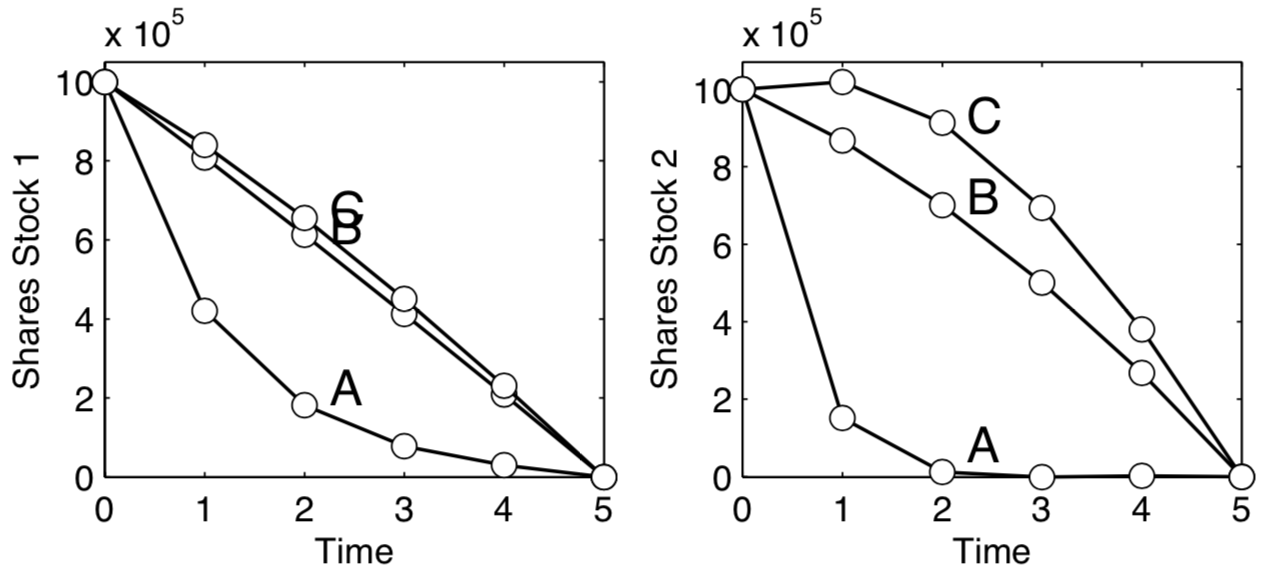
\includegraphics[width=\textwidth]{chapters/chapter_exec_models/figures/opt_traj.png}
	\caption{Optimal Trajectories for two securities; ($A: \lambda= 2 \times 10^{-6}$; $B: \lambda=0$; $C= -5 \times 10^{-8}$; $B$ is the na\"ive strategy). \label{fig:7first}}
	\end{figure}
	\begin{figure}[!ht] 
	\centering
	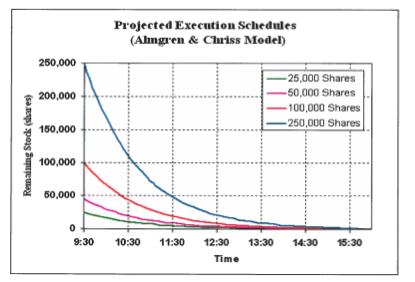
\includegraphics[width=\textwidth]{chapters/chapter_exec_models/figures/temp2.png}
	\caption{Projected Execution Schedules \label{fig:7second}}
	\end{figure} \todo{nonscanned version?}
 

Some questions remain: what is the link between market impact and the dynamics of limit order book, is the impact function linear empirically, etc.. The effect of a short term drift in prices and the serial correlation in the errors which is observed in high frequency etc can be incorporated easily in the model \eqref{eqn:morepk}. Lorenz and Almgren (2011)~\cite{lovenz2011} provide a Bayesian approach to the optimization problem. While the methodology yields elegant solutions, empirical use of these results require a close monitoring of order book dynamics as the changes in demand and supply sides can be quite rapid. The general behavior of this adaptive strategy is aggressive; it depends on the prediction of short term price change; generally, if price goes up sell faster. 


The above mean-variance formulation of execution cost is combined with the traditional mean-variance portfolio optimization in Engle and Ferstenberg (2007)~\cite{engle2007} and Engle, Ferstenberg and Russell (2012)~\cite{engle2012}. We will discuss this in the context of portfolio rebalancing and the need for minimizing the transaction costs associated with all trades. While the above methods can be taken as first generation methods that are purely based on slippage, more recent work focus on adding other constraints such as incorporating the market VWAP and simultaneously determining the limit and market orders to achieve optimal results. \\


\noindent\textbf{Obizhaeva and Wang Model:} The models discussed in the previous sections assume price impact function that is not sensitive to liquidity dynamics. Obizhaeva and Wang (2013)~\cite{obizhaeva} develop a model that accounts for the dynamic properties of supply and demand as represented in the limit order book. The model captures `resilience'; that is, how the current trade affects the state of the future limit order book. The resulting strategy consists of a large trade initially aimed at moving the order book away from its steady state followed by a number of small trades that will utilize the inflow from new liquidity providers. The speed at which the book replenishes itself is an important part of execution cost. The level of resilience depends on the level of hidden liquidity in the market. The price impact model considered here takes into account the dynamics of the limit order book.


It is assumed that the parent order $X$ will be traded in the interval $(0,T)$, `$n$' times at $t_1, t_2, \ldots, t_n$. To model the execution of a large order in the limit order book, it is assumed that the price of execution ($p_t$) depends on the true value of the equity ($p_t^*$) and the state variables ($z_t$) such as past trades that may affect the book. Let $q(p_t^*,p_t;z_t)$ be the density of the limit orders in the other side of the book. The mid-quote ($\overline{p}_t$) is generally taken to reflect the true price, $p_t^*$. If the trade is on the buy side, the initial large transaction, $x_1$, can push the ask price to a higher level, $p_1^* + (s/2) + (x_1/q)$, where `$s$' is the spread and the average execution price is then equal to $p_1^* + (s/2) + x_1/(2q)$. After the initial execution the price converges to a new steady state, $p_t^*+s/2+\lambda x_1$. Assuming that the limit-order book converges to its steady-state exponentially and at time `$t$', 
	\begin{flalign} \label{eqn:qtdouble}
	&& q_t(p)&= q\cdot I(p>A_t) && \notag \\
	\text{and} && \phantom{x} & \phantom{x} && \\
	&& A_t&= \overline{p}_t + \dfrac{s}{2} + x_1 \cdot \kappa e^{-\rho t}, && \notag
	\end{flalign}
where $A_t$ is the asking price, $\kappa= 1/q - \lambda$ and `$\rho$' measures the resilience of the limit order book. If more the current ask price ($A_t$) deviates from steady state level, $\overline{p}_t + s/2$, the new ask limit orders will come into the book as the rate of $\rho \,q \,(A_t - \overline{p}_t - s/2)$. 


Given the above description of the limit order book dynamics, the optimal execution problem can be restated as follows:
	\begin{equation} \label{eqn:min}
	\min_{x_k} E_1\left( \sum_{k=1}^n [A_k + x_k(2q)] \,x_k \right),
	\end{equation}
such that $A_k= p_k^* + \lambda(X_1-X_n) + \dfrac{s}{2} + \sum_{i=1}^{k-1} x_i\ cdot \kappa e^{- \rho \tau(n-i)}$, where $p_k^*$, the true price is taken to follow a random walk.


The solution to this dynamic programming problem is given in Obizhaeva and Wang (2013)~\cite[p.14, Proposition 1]{obizhaeva} and is somewhat involved. Instead we state, the strategy when $n \to \infty$ which is of practical interest as many parent orders are divided into many, many child orders. The empirical market impact study that was presented in the last chapter attests to that. The solution to \eqref{eqn:min} as $n \to \infty$ are:
	\begin{equation} \label{eqn:orders}
	\begin{split}
	\text{First and final orders}: x_1&= \dfrac{X}{\rho_{T+2}} = x_n  \\
	\text{Spread of in-between trading}: x_t&= \dfrac{\rho x}{\rho_{T+2}}.
	\end{split}
	\end{equation}
The expected cost is determined as
	\begin{equation} \label{eqn:expected}
	\text{Expected cost}= \left( p_0^* + \dfrac{s}{2} \right) X_t + \lambda X_0 X_t + \alpha_t X_t^2 + \beta_t X_t D_t + \gamma_t D_t^2,
	\end{equation}
where $\alpha_t= \dfrac{\kappa}{\rho(T-t)+2} - \dfrac{\lambda}{2}$, $\beta_t= \dfrac{2}{\rho(T-t) + 2}$ and $\gamma_t= - \dfrac{\rho(T-t)}{2 \kappa[\rho(T-t) + 2]}$. The initial and final orders are discrete in nature and the orders in-between are continuous. They make use of incoming orders with favorable prices. 


Some comments are worth noting. Note the solution given in \eqref{eqn:orders} does not depend on the market depth, `$q$' and the price impact, `$\lambda$'. It is shown that the price impact is not a factor if the trade times are determined optimally and if they are not set a priori as in the other strategies. The reason for `$q$' not being a factor is due to the fact that the depth is taken to be constant at all times. This implies that there is enough liquidity in the market and the book gets replenished, albeit at a constant rate. The two factors that play important roles are the resiliency factor, `$\rho$' and the trading horizon, `$T$'. When $\rho=0$ the execution costs are strategy dependent and when $\rho \to \infty$, the order book rebuilds itself faster. When `$T$' increases, the size of the first and final order decreases; if there is more time to trade, the trades are spread out to manage the execution cost. The net cost of this strategy is
	\begin{equation}\label{eqn:netcost}
	\text{Net cost}=\dfrac{\lambda}{2} \cdot X^2 + \left(\dfrac{\kappa}{\rho_{T+2}}\right)^2 X^2
	\end{equation}
and it is shown to be smaller than the cost incurred if the strategy of constant rate trading is followed. 


Obizhaeva and Wang (2013)~\cite{obizhaeva} consider the extension of the optimization criterion in \eqref{eqn:min} to include the risk aversion as well, as in Almgren and Chriss (2000)~\cite{alm2000}. Interested readers should refer to Section~8 their paper. For a practical implementation of these methods, it is necessary to consider the trading that happens in multiple exchanges and how the replenishment patterns can differ over different exchanges where `liquidity' and the fee structure have become major considerations for the order flow. 


\noindent\textbf{Easley, De Prado and O'Hara Model:} In the models described so far in this section, it is assumed that the number of child orders `$n$' and the execution horizon, `$T$', are decided exogenously. Also the impact of a trade is modeled through the modified random walk model for the price with additional terms reflecting the permanent or temporary impact (Equations \ref{eqn:pk7}, \ref{eqn:bigpk} and \ref{eqn:pdouble}). The process of how price impact arises due to friction in the liquidity access is an important part of market microstructure theory and this needs to be taken into account in determining the optimal execution. For example, a buyer in a seller's market can incur a lower cost of trading than a seller in a similar market. Obizhaeva and Wang model is based on the arrival dynamics to the order book. 


The approach taken by Easley, De Prado and O'Hara (2015)~\cite{prado2} is based on an asymmetric information model of the market maker's behavior. The key measure is the probability of information-based (PIN) trading that is estimated by the order book imbalance (see Easley, De Prado and O'Hara (2012)~\cite{prado3}). Selling a large order in a market already imbalanced toward sell, will reinforce adverse selection from the other side and thus widen the bid-ask spread resulting in higher market impact. The optimal execution horizon (OEH) model in Easley et al (2015) provide a framework for determining the trading horizon, `$T$', and does complement other earlier studies on execution strategies that minimize the price impact. 


The PIN that was developed in a series of papers (see Easley, Kiefer, O'Hara and Paperman (1996)~\cite{paper} and the references therein) views trading as a sequential game between liquidity providers and liquidity takers, repeated over the trading duration. If the information about the asset occurs with probability $\alpha$ and the chance that the information is good, is denoted by, $(1 - \delta)$ and further assume that the informed traders, who knew the terminal value of the asset under good news ($\overline{S}$) and under bad news ($\underline{S}$) arrive at the rate, $\mu$, and the noise traders arrive at the rate of `$\epsilon$'. The PIN is approximated as (assuming $\delta= 1/2$)
	\begin{equation} \label{eqn:pin}
	\text{PIN}= \dfrac{\alpha\mu}{\alpha\mu + 2\epsilon} \sim E[\text{OI}],
	\end{equation}
where order imbalance (OI), ($\text{OI}= \frac{V^B - V^S}{V}$), with $V$ denoting the volume. An aggressive buy order of size `$m$' can affect the order imbalance as
	\begin{equation} \label{eqn:oi}
	\text{OI}=\left( 2 \cdot \dfrac{V^B}{V} - 1 \right) \left(1 - \dfrac{m}{V} \right) + \dfrac{m}{V},
	\end{equation}
and note that $\left( 2 \cdot \frac{V^B}{V} - 1 \right)$ is the order imbalance, when $m= 0$, that is without the large trade. When `$m$' is small, the OI is likely to be perturbed too much and $m \to V$, that is the buy order will take all the available liquidity, then $\text{OI} \to1$. This also indirectly quantifies the amount of leakage or signaling that occurs with each trade.


An important factor that is associated with PIN is the range of liquidity that may exist in the market in the presence of both informed and noise traders:
	\begin{equation}\label{eqn:newsigma}
	\Sigma = \text{PIN} \cdot [\overline{S} - \underline{S}]
	\end{equation}
slicing a large order into small orders as suggested by earlier execution strategies does have timing risk and the asset price is assumed to follow a random-walk resulting in:
	\begin{equation}\label{eqn:randomwalk}
	\Delta S= \sigma \sqrt{\dfrac{V}{V_\sigma}} \, \xi,
	\end{equation}
where $\xi \sim N(0,1)$, $V_\sigma$ is the volume in the mid-price range. With `$\lambda$' as the probability of accepting a loss greater than $z_\lambda \cdot \sigma \cdot \sqrt{V/V_\sigma}$, the loss from trade size, `$m$', can be shown to be bounded by,
	\begin{equation}\label{eqn:bigbracp}
	P \left[ \dfrac{m \cdot \Delta s}{\hat{\sigma} \sqrt{\dfrac{V}{V_\sigma}}} > z_\lambda \right] = 1-\lambda
	\end{equation}
and thus `$\lambda$' can be interpreted as a `risk aversion' parameter. The OEH's goal is to determine the optimal trading volume, $V$, that can hide the purported trade, $m$, with minimum timing risk. The probabilistic loss function $\Pi$ that incorporates both liquidity and timing risk component is defined as:
	\begin{equation}\label{eqn:pi}
	\Pi = \left| \varphi(m) \cdot \text{OI} + (1-\varphi(m)) (2V^B-1)(\overline{S}-\underline{S})\right| - z_\lambda \sqrt{\dfrac{V}{V_\sigma}} \, \sigma.
	\end{equation}
Here $\varphi(m)$ is a monotonic function that maps into the range $(0,1)$. If `$V$' is greater, its impact is smaller in OI and larger in the trading range. The optimization results are given in Easley et al (2015)~\cite{prado2}.


The key quantities in determining the OEH are the order imbalance and the trade size/side. Figure~\ref{fig:3temp}, reproduced from Easley at al demonstrates how selling in a buyer's market allows for shorter horizons and in seller's market leads to longer horizons.  


        \begin{figure}[!ht] 
        \centering
        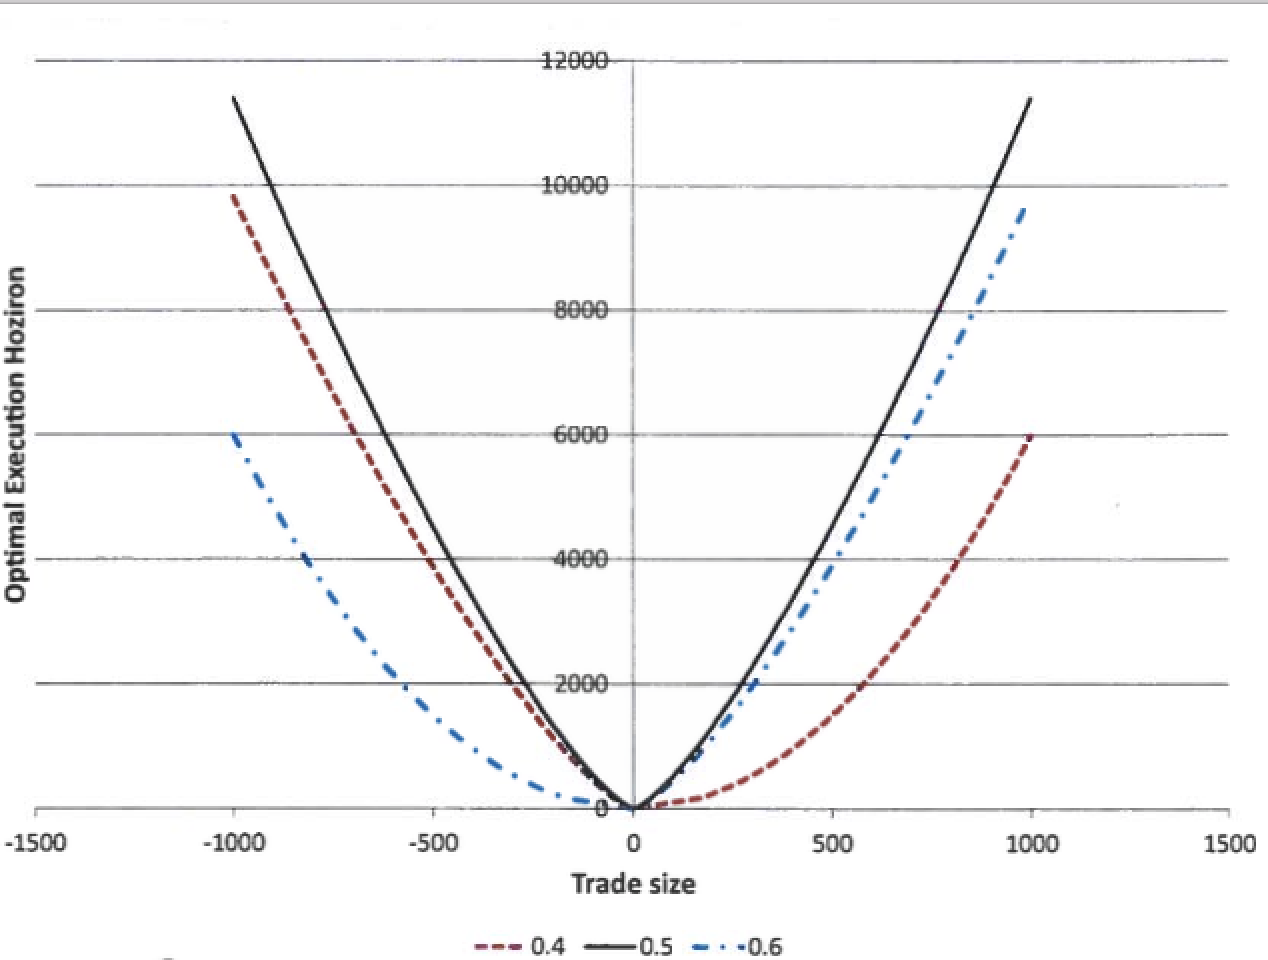
\includegraphics[width=\textwidth]{chapters/chapter_exec_models/figures/fig3temp.png}
         \caption{Optimal execution horizons for various order imbalances and trade sizes/sides. Combining alternative trade sizes and sides with our three scenarios ($v^B=0.4$, $v^B=\frac{1}{2}$, $v^B=0.6$) results in the optimal execution horizons displayed in the figure above, $\hat{\sigma}=1,000$, $V_\sigma=10,000$, $m=1,000$, $[\overline{S}-\underline{S}]=10,000$, $\lambda=0.05$ and $\varphi[|m|]$ linear. \label{fig:3temp}}
        \end{figure} \todo{nonscanned version?}



% Multiple Exchanges:  Smart Order Routing
\subsection{Multiple Exchanges:  Smart Order Routing}


In the USA there are over ten lit venues and close to forty dark venues and thus equity markets are highly fragmented. Each venue functions as an electronic limit order book of its own, where orders are prioritized first based on their prices and then at a given price level, according to their time of arrival. Exchanges publish information for each security in real-time and the information can change rapidly due to cancellations. The exchanges may differ with respect to best bid and offer price levels, the market depth at various prices etc. The exchanges also differ in their fee structures. Under the maker-taker pricing, exchanges offer rebates to liquidity providers and charge fees to takers of liquidity. These fees can range from $-\$0.001$ to \$0.0030. Because the typical bid-ask spread is \$0.01, the fees and rebates are a fairly significant fraction of the trading costs. Thus market participants must decide where child orders should be sent. It may be expensive to route to all the exchanges and by not routing to the right venue, it is possible to miss liquidity and hence incur greater market impact. At any point in time, the highest bid and the lowest offer among all exchanges comprise the National Best Bid and Offer (NBBO). Most traders use the smart order routing algorithms with goal to buy or sell the maximum number of shares in the shortest possible time with the least market impact possible. But a key issue is that many of the lit venues have hidden orders (12--45\%). How to estimate the size of the hidden orders and how to make routing decisions in the presence of hidden orders has been a focus of some recent research studies.


While exchanges compete along many fronts, for example, payment for order flow, transparency and execution speed, the key variables driving the efficiency are liquidity and price improvement. Thus the design of market structure is considered by market participants and regulators as the key determinant of flow of liquidity. The coexistence of multiple exchanges as mentioned in Parlour and Seppi (2003)~\cite{parlour2003} raises specific questions that are stated below:
        \begin{enumerate}[a)]
        \item Do liquidity and trading concentrate in a few exchanges?
        \item Do some market designs provide greater liquidity than others?
        \item Is the fragmentation of order flow desirable from a policy point of view?
        \item What is the constructive role for regulators to enhance liquidity?
        \end{enumerate}


Because exchanges operate under rules governing certain market designs, the performance and efficiency issues are related to the types of markets, such as pure limit order and a hybrid market (limit order book plus a specialist). In the hybrid market a specialist can provide supplementary liquidity after a market order has arrived. Parlour and Seppi (2003)~\cite{parlour2003} conclude only under some conditions such as enforcement of time priority, the efficiency is possible. Merely increasing the number of trading venues may result in degradation of market quality, if the enforcement of time priority is not followed, as it might discourage traders from posting the limit orders.


Foucault and Menkveld (2008)~\cite{foumen}consider the effect of fragmentation on two limit order markets. They examine the competition between Euronext and London Stock Exchange (LSE) in the Dutch market. The consolidated limit order book is found to be deeper after entry of the LSE. General conclusions from the above study and others such as Hendershott, Jones and Menkveld (2011)~\cite{hjm} and O'Hara and Ye (2011)~\cite{oye} are that fragmentation of order flows improves the liquidity supply and protecting orders against trade-throughs is important. Thus multiple exchanges are here to stay and smart order routing algorithms that can work well with the increased number of exchanges would be favorably sought by the market participants.


The smart order router (SOR), generally works as follows. A user can customize the use of the strategy by establishing a set of rules in splitting the parent order into child orders and the smart order routers are designed to ensure that the orders are routed to the venue with the best price and the orders are filled according to the trading strategies that may be pre-determined or may be adaptive. To be successful, SORs must be able to handle a variety of trading strategies and multiple venues. In addition they must deal with vast amount of incoming and historical market data. The publicly available information on the SORs used by major traders indicate that the order placement objective in general is to minimize client all-in shortfall with or without venue fees. The all-in shortfall consists of the shortfall on the filled shares and the cost of the clean-up trade for the unfilled shares. The latter is taken to be an important component of order placement optimization as it enables to quantify the effect of venue differences in fill rates, (see Street Smart, Issue 42, Jan 14, 2011). Other programs used in industry chose to optimize the expected time to execute the client's overall order. Expected queue speeds at various venues are predicted from recent trading data. Small orders tend to be placed in a single venue to minimize the queueing time whereas large orders will be placed in multiple venues to access maximum liquidity. In this model forecasting trading rates at different venues is crucial for successful implementation of the program. The rates are modeled as a function of lagged rates, thus capturing the momentum, and imbalances between supply and demand sides of the order book. Thus order placement in a fragmented market is not a trivial task.


A recent empirical study by Battalio, Corwin and Jennings (2016)~\cite{battcorjen} confirms that brokers use both limit and marketable orders to execute trades. Past studies provide evidence that market orders are sent to venues with lower trading costs and the trading fees and rebates generally affect consolidated market depth. Maglaras, Moallemi and Zheng (2012)~\cite{magmoazhe} show that limit orders are submitted to exchanges with high rebates and lower waiting time for execution while market orders are sent to venues that have lower fees and larger posted quote sizes. Cont and Kukanov (2017)~\cite{contk} develop a model that is somewhat more realistic to the current practice by decoupling the `order placement' decision from the scheduling decision and more importantly consider the option of placing limit orders on several exchanges, simultaneously. The model also accounts for the execution risk, the risk of not filling an order. Filling the unfilled portion may be costly and the allocation may shift toward market orders or toward overbooking, that is placing more orders than needed to refill.


To formalize the order placement problem, we assume a size of order $X$ is to be filled in the duration $(0,T)$. The decision is to split this order into a market order $M$ and `$K$' limit orders $L_1, \ldots, L_K$ with the same size to be placed in `$K$' exchanges with queue sizes $Q_1, \ldots, Q_K$ ; thus the order allocation is summarized by the elements of the vector $X=(M, L_1, \ldots, L_K)$ that need to be optimally determined. If order cancellations in the duration $(0,T)$ in exchange `$K$' is represented by $\xi_K$, then the number of shares transacted can be written as 
	\begin{equation} \label{eqn:axe}
	A(X,\xi)= M + \sum_{k=1}^K \left[ (\xi_k - Q_k)_+ - (\xi_k - Q_k - L_k)_+ \right],
	\end{equation}
where the terms in the parenthesis refers to the initial position and the final position of the queue outflows. The execution cost must account for fee ($f$) and rebate structures (discussed in Chapter~\ref{chap:ch_mi_models}) in each exchange and the cost of adverse selection ($r_k$) and can be stated as follows:
	\begin{equation}\label{eqn:cxe}
	C(X,\xi)= (h+f) M - \sum_{k=1}^K (h+r_k) \left[ (\xi_k - Q_k)_+ - (\xi_k - Q_k - L_k)_+ \right].
	\end{equation}
Here $h$ is one-half of bid-ask spread. 


The cost function in \eqref{eqn:cxe} can be modified to account for the cost of unfilled limit orders which may be filled through market orders at higher cost or it is possible that the prices have decreased resulting in additional adverse selection cost with penalty ($\lambda_u$) for falling behind and penalty ($\lambda_0$) for exceeding the target; Thus, the execution risk can be written as,
	\begin{equation}\label{eqn:er}
	\text{ER}= \lambda_u (S-A(X,\xi))_+ + \lambda_0 (A(X,\xi)-S).
	\end{equation}
To be more realistic, the market impact function can be considered as follows:
	\begin{equation}\label{eqn:mi}
	\text{MI}= \theta \left[ M + \sum_{k=1}^K L_k + (S-A(X,\xi))_+ \right].
	\end{equation}
The total cost function that includes both implicit and explicit costs can be states as:
	\begin{equation}\label{eqn:vxe}
	V(X,\xi)= C(X,\xi) + \text{ER} + \text{MI}.
	\end{equation}
The random variable in \eqref{eqn:vxe} is $\xi$, the cancellations that occur in various exchanges and the minimization function is $E[V(X,\xi)]$ with some assumed distribution for $F$ of $\xi$. Under some reasonable assumptions such as that the trader will not execute more than the target $X$ and market orders in the beginning of the duration $(0,T)$ are less expensive than at the end when unfilled orders are converted to market orders, an optimal solution is shown to exist (see Cont and Kukanov (2017)~\cite{contk} for details).


The analytical solution minimizing $V(X,\xi)$ is not easily tractable due to dimensionality issues. A numerical solution via gradient method is proposed. Random samples of $\xi$ are obtained and averaged to approximate $E(\xi)$. Let $q(X,\xi)= \Delta V(X,\xi)$ be the gradient of $V$. The following iterative algorithm is shown and converges:
	\begin{enumerate}[--]
	\item \textbf{Start with }$\mathbf{X_0}$\textbf{ and for }$\mathbf{n=1,2,\ldots,N}$\textbf{ do}
	\item $\mathbf{X_n=X_{n-1} - \gamma_N g(x_{n-1}, \xi^n)}$
	\item \textbf{End; }$\mathbf{X_N^* = \frac{1}{N} \sum_{n=1}^N X_n}$
	\end{enumerate}
The step size, \small
	\begin{equation} \label{eqn:7gammaN}
	 \gamma_N = \sqrt{k} S \left( N(h+f+\theta+\lambda_u +\lambda_0)^2 _ t + N \sum_{k=1}^K (h+r_k+\theta+\lambda_u+\lambda_0)^2 \right)^{-1/2} 
	\end{equation}
can be seen as a function of all the costs associated with the execution of the order.


To summarize, recall that the algorithm needs the following input:
	\begin{enumerate}[--]
	\item Trading Costs: 
		\begin{itemize}
		\item One half of bid-ask spread ($h$)
		\item Market order fee ($f$)
		\item Effective limit order risks ($r_k$)
		\item Market impact coefficient ($\theta$)
		\item Penalties for overfilling or underfilling ($\lambda_0,\lambda_u$)
		\end{itemize}
	\item Market Variables: Number of exchanges ($K$) and limit order queues ($Q_k$).
	\item Execution Variables: Time horizon ($T$) and target quantity ($S$).
	\end{enumerate}
While many of these quantities can be estimated using past transactions, the limit order queues ($Q_k$) and the cancellations ($\xi_k$) are to be obtained at the time of execution.



\subsection{Algorithmic Trading Next Frontiers}
\noindent\emph{ Stochastic Adaptive Control Approach to Optimal Execution}
\noindent\emph{Reinforcement Learning}
\section{The Future of Execution Strategies}